\documentclass{article}

% NeurIPS 2026 Evaluations and Datasets track. [preprint] for the arXiv
% version; drop the option for an anonymized submission, [final] for camera
% ready.
\usepackage[preprint]{neurips_2026}

\usepackage[utf8]{inputenc}
\usepackage[T1]{fontenc}
\usepackage{microtype}
\usepackage{amsmath,amssymb}
\usepackage{booktabs}
\usepackage{siunitx}
\usepackage{graphicx}
\usepackage{subcaption}
\usepackage{xcolor}
\usepackage{enumitem}
\usepackage[hidelinks,breaklinks]{hyperref}
\usepackage[capitalise,noabbrev]{cleveref}

\sisetup{
  table-format = 1.4,
  % Print each cell exactly as written: every cell already carries its intended
  % precision, and rounding to places padded three-decimal values to four.
  round-mode = none,
  detect-weight = true,
}

\graphicspath{{figures/}}

\newcommand{\passk}{\text{pass}^{k}}

\title{SharpeArena: A Deterministic Point-in-Time Evaluation Sandbox and Reinforcement-Learning Environment for Trading Agents}

\author{%
  Tiberiu Toca \\
  General Liquidity \\
  \texttt{tibi.toca@gmail.com}
}

\begin{document}

\maketitle

\begin{abstract}
Reinforcement-learning results in trading are produced by the party being evaluated, on an environment that party controls and defends as realistic on the strength of its frictions: transaction costs, slippage, position limits. Frictions constrain the agent, and say nothing about whether the simulated world behaves like a market or about whether the trajectory the environment emitted is the one it ran. We present SharpeArena, a deterministic point-in-time evaluation sandbox and reinforcement-learning environment for trading agents. It excludes three failures at the interface rather than discouraging them: no data-layer operation returns a bar past the engine's cursor, committed canonical fixtures and fingerprints pin the determinism-critical core across tested surfaces, and replay recomputes performance from recorded decisions and frozen engine inputs, so a doctored decision stream produces a different run. Agents are external programs, language models included, that reach the engine through a governed JSON contract. A host-side parser enforces episode semantics, and the checked scoring paths record a wire fault as a typed failed cell rather than as a hold. Around that loop the environment adds a strategy-generation path over a closed non-executable candidate language, a forward paper-trading arm, and prospective forecast contracts that freeze the target, information boundary, deadline, resolution rule and score before submission. Forecast revisions remain append-only, and the producer exports raw evidence for the separate SharpeBench kernel to score without affecting trading rank. Selected deadline, revision, binding and fixed-point Brier rules are modeled in Lean; separate executable tests check the same rules against the implementation, and nothing mechanically links the model to the code. We calibrate the environment's diagnostics with fixed reference policies: nothing is trained and no admitted result is a claim about model quality. The generalization protocol is therefore demonstrated rather than exercised, and the obstacle is a learner's training cost rather than environment time, since the slowest shipped surface runs ten million steps in about twelve minutes. The committed F1--F8 artifacts were produced before most current engineering guards, F7 alone having been regenerated for release 0.29.0, and a superseded convenience-sample protocol pilot produced no admitted model-validation result. We find that the canonical generator fails its own realism diagnostic on 23 of 24 seeded panels, that a predeclared sweep of its volatility-clustering knobs finds no Calm setting that survives, that no reference policy is rank-eligible, and that a single-seed reading of the ecology probe does not survive replication. We offer a producer whose current guarantees are properties of committed code rather than of its authors' good faith, and diagnostics that report where its historical tape is not yet market-like.
\end{abstract}

\section{Introduction}\label{sec:intro}

Every published number in agent trading evaluation is produced by the party being evaluated, on an environment that party controls. Three failures upstream of scoring void any score, and none of them is visible in the score itself. An agent that observes one future bar has an edge no deflation can remove; look-ahead bugs are a pervasive and usually invisible failure mode of backtests, alongside the selection bias the deflation literature centers \citep{bailey2014deflated}. \Citet[p.~7]{gencay2026honest} shows the first point directly: a deliberately leaky oracle posts a deflated Sharpe ratio of 1.00, because deflation has no mechanism against a strategy whose information set is contaminated. Authors of recent systems have found such leaks in their own pipelines only after a result looked implausible, one through a manual audit of an implausible held-out score that a model reviewer had let pass \citep[pp.~21--22]{guo2026aqua}, another after an off-by-one date slice had put validation-year labels into training and inflated test Sharpe by 0.3 \citep[p.~11]{du2026mlfactor}. An environment that is not bit-reproducible cannot support a leaderboard, because the same submission scores differently on different machines and no one can check anyone else's number. And a trajectory that cannot be recomputed from the environment that allegedly produced it is a self-reported claim, not evidence.

We use \emph{evaluation sandbox} to mean a controlled market interface with governed observations, actions, replay, and evidence. The term does not imply operating-system, process, or container isolation; \cref{sec:limitations} states that separate boundary explicitly.

The trading environments agents are trained and evaluated on close none of the three, and the realism they do claim is claimed on a different axis. FinRL states that it replicates the live stock market and cashes that statement out entirely as frictions: transaction cost, liquidity and risk aversion \citep{liu2020finrl}. TradeMaster likewise incorporates practical constraints such as transaction costs, slippage and a non-negative balance in the name of a more realistic environment, defers its transition function to FinRL-Meta by citation, and reports backtest metrics where a validation of the simulated market would go \citep{sun2023trademaster}. ABIDES claims high fidelity in its title and asserts that its platform produces realistic slippage naturally, without quantitative evidence for either \citep{byrd2020abides}; ABIDES-Gym inherits those background-agent configurations without revalidating them and acknowledges only rare unrealistic behavior in the synthetic market \citep{amrouni2021abidesgym}. FinRL-Meta is the honest exception: it names the sim-to-real gap and enumerates what it leaves unmodelled, including permanent market impact of limit orders and a non-resilient limit order book, though it quantifies none of it and tests no distributional property of returns \citep{liu2022finrlmeta}. mbt\_gym makes no realism claim at all; it claims correctness and demonstrates it by recovering a known closed-form optimum \citep{jerome2023mbtgym}, which is verification rather than validation, and is honest precisely because it never conflates the two. The language-model trading literature has the same gap. A 2025 survey observes that the growth of financial language models has outpaced standardized, time-safe benchmarks that connect text to tradable decisions, and that agent frameworks report simulation results on internal market environments, with little standardization of latency, slippage, queue priority or order mix \citep[pp.~11--12]{fu2025newquant}.

Read together, the pattern is a substitution: frictions stand in for dynamics. A friction bounds what the agent is allowed to do. It carries no information about whether the process the agent acts on behaves like a market, and none at all about whether the trajectory the environment reports is the one it ran. SharpeArena addresses both halves of what the substitution leaves out: the three producer failures above are excluded structurally, and the question of whether its own tape is market-like is asked as a committed diagnostic that the canonical generator currently fails (\cref{sec:f4}). \Cref{sec:related} makes the comparison on the five property axes.

The companion SharpeBench paper \citep{toca2026sharpebench} supplies the scorer that consumes these trajectories: it argues that ranking trading agents on raw return over short windows measures luck, and its deterministic kernel deflates for search breadth \citep{bailey2014deflated}, gates on per-run reliability \citep{yao2024taubench}, and zeroes entries that bypass risk controls. Every one of its guarantees is conditional on the trajectory being honest, which is the problem this paper takes.

SharpeArena excludes each of the three failures at the environment's own interface, then adds a detection layer behind the structural guarantee for defense in depth. Look-ahead is prevented by the shape of the data layer, which has no API that returns a future bar, and additionally policed by a deny-list guard at the harness boundary; this is an interface guarantee, and \cref{sec:limitations} states what it does not cover, including in-band prediction of the public deterministic generator. Determinism is achieved by restricting the scenario generator's arithmetic to operations that are exact and identical on every platform, and additionally pinned by committed golden hashes checked in continuous integration on native, WebAssembly and packaged Python surfaces. Trajectory verification records decisions and recomputes performance from them and the frozen engine inputs. A tamper test changes the decisions and requires the replayed run to diverge; fields outside that replay input are not thereby authenticated.

A fourth failure appears only once the agent is a separate process rather than a Python object, which is the arrangement a language-model agent forces. The transports that carry a decision over a wire have no way to report a wire fault through the interface they implement, so a timeout or a dropped connection arrives as an empty decision, and an empty decision against a stateful engine is a hold that persists the position. A wedged agent therefore completes its window and emits a return series that no scoring gate can distinguish from a deliberately conservative one, because every gate consumes returns. \Cref{sec:transport-gate} converts a recorded fault into a typed failed cell instead, and \cref{sec:agentic} applies the same rule to the two other places the agentic layer can silently substitute a plausible default for a fact it does not have.

The interface follows the pattern that made Gym the substrate of a decade of reinforcement-learning research \citep{brockman2016gym,towers2024gymnasium}: a small, stable boundary that outlives any single environment behind it. An agent is a program in any language that reads a JSON \texttt{Observation} and writes a JSON \texttt{Decision}. The contract is versioned, additive-only, schema-published and governed by a written deprecation policy, so a vendor can build against it once. Conform to the contract and you are scorable everywhere the SharpeBench kernel runs. Whether an ecosystem forms around this contract is an adoption question the paper does not answer; \cref{sec:limitations} records that no third party has yet submitted an agent.

\paragraph{Scope and contribution boundary.} This paper claims the environment, its agentic layer and its protocol: the interface-level leak-freedom, the cross-runtime determinism, the replay verifiability, the wire contract and the fault typing on it, the strategy-generation, prospective-forecast and forward-execution paths, the seed-band generalization protocol, and the probe layer, together with the calibration experiments that exercise them. The scoring semantics, the deflation prior and the dispersion-unit bug that SharpeBench 0.3.0 fixed are the companion SharpeBench paper's contributions \citep{toca2026sharpebench}; F1 appears here only as validation that the producer-scorer separation catches scorer bugs. Two absences are separate and both belong here rather than in a late caveat. No agent is trained in this paper: every F1--F8 experiment uses fixed reference policies, and a learning baseline through the shipped Gymnasium adapter is named future work in \cref{sec:limitations}. No current-model field has been completed or admitted either. A superseded engineering pilot using obsolete convenience-sample checkpoints remains committed for protocol auditability, but it is excluded from the paper's results and from benchmark rank. The agentic layer of \cref{sec:agentic} is therefore claimed as architecture with verifiable guarantees, not as evidence of model performance, and no third party has submitted an agent (\cref{sec:limitations}). The empirical artifacts, archived engineering traces and present guarantees are distinct provenance classes (\cref{app:commands}).

\paragraph{Contributions.}
\begin{enumerate}[leftmargin=*,itemsep=2pt]
\item A point-in-time (PIT) reinforcement-learning environment for trading agents that is leak-free at its interface boundary, cross-runtime byte-deterministic in its Rust core, and decision-replay-verifiable, with readable canonical pre-hash fixtures, a cross-wrapper tape-semantics fingerprint and effective-configuration readback identifying the enforcing code and the boundary of each property.
\item A governed agent wire contract at version 1.0 with JSON Schemas, conformance fixtures and an additive-only evolution policy. It is the boundary an external program, a language model included, crosses to reach the engine, and it carries the fault typing of the next item.
\item Fault typing on the scored path. A transport fault is converted into a typed failed cell rather than the empty-orders hold the transports emit, because against a stateful engine that hold persists the position and produces a return series indistinguishable from a conservative agent's (\cref{sec:transport-gate}). The same rule makes an unknown paper submission a representable state rather than a guessed one (\cref{sec:forward-paper}), and records the decisions that were refused alongside the ones that executed (\cref{sec:counterfactual}).
\item An evidence-admissibility discipline for the agentic layer: a closed falsifiability manifest binding each generated candidate to a hypothesis, a mechanism, invariants and quantitative kill conditions, recorded with a host-counted trial ordinal before validation (\cref{sec:edge-manifest}); and a strict silver-to-gold promotion path that refuses malformed production traces rather than skipping them (\cref{sec:trace-promotion}).
\item A procedural scenario generator with disjoint train, gap and held-out seed bands in the Procgen tradition \citep{cobbe2020procgen}, making the generalization gap a measured quantity for any policy submitted to it. No learner is measured here, so what this paper establishes is the apparatus and its resolution rather than a learner's generalization gap. The only gap it reports is for a fixed parameter-free policy that has nothing to overfit, and that gap reads near zero by construction (\cref{sec:f3,sec:limitations}).
\item A task suite that includes a market-making environment shipping the analytical Avellaneda--Stoikov quoting policy \citep{avellaneda2008high,gueant2013dealing} as a reference, so agents are scored on regret against a fixed analytical baseline rather than against each other.
\item A diagnostic layer that probes realism, manipulation payoff boundaries, adverse-selection markouts, population ecology and generator predictability. Two opt-in paths extend it: a concave-impact path that leaves the canonical linear golden path byte-identical, and a sealed-seed derivation that hides the held-out seeds behind a commit--reveal salt while the seed-band structure keeps disjointness from the train band checkable by construction, without the salt.
\item A prospective forecast-evidence protocol that freezes settlement and scoring semantics before submission, records eligible, rejected and late revisions append-only, binds information exposure, and exports an unscored strict artifact for SharpeBench. An executable cross-product tutorial exercises the boundary without a package cycle. A separate Lean model proves selected deadline, revision, binding and fixed-point Brier properties, and executable tests check the same rules against the implementation independently; no mechanism links the model to the code (\cref{sec:prospective-protocol}).
\item The executed experiments and follow-ups of \cref{sec:validation,sec:findings}, in which every number is produced by a committed script listed in \cref{app:commands}.
\end{enumerate}

\paragraph{What the evidence shows.} Every finding is an instrument calibration on canonical tape that fails the finite-panel-calibrated realism conjunction in 23 of 24 seeded panels, and a predeclared Calm calibration sweep finds no setting that survives its diagnostic, confirmation and volatility rule (\cref{sec:f4,sec:calm-tails}). Under the corrected kernel no reference policy is rank-eligible (\cref{sec:f1}), yet a common-random-number oracle witness attains eligibility on every tier and finds the per-run reliability gate, which requires every seed's probabilistic Sharpe ratio (PSR) \citep{bailey2012sharpe} to clear its bar, last to open at every attained crossing (\cref{sec:witness}); \cref{sec:f1} states the Sharpe-ratio convention these statistics use. The manipulation, adverse-selection, predictability and ecology probes each report against the environment as often as for it, and \cref{sec:validation,sec:findings} state the scope of each. What the evidence does not show belongs here rather than only in \cref{sec:limitations}. Without a positive control on tape known to be market-like, the realism verdict establishes that this gate refuses this generator and not that the gate discriminates (\cref{sec:f4}). The generalization gap of \cref{sec:f3} is reported only for a parameter-free policy, so that section demonstrates the measuring apparatus and not a learner's gap.

\section{Design principles}\label{sec:principles}

Every decision in the environment traces to one of eight principles.

\textbf{Leak-free at the interface.} The environment owns the time cursor, and the data layer exposes no operation that returns a bar after it. An agent cannot peek through the interface because there is nothing to call, not because a rule forbids it. Detection layers exist, but they sit behind the structural guarantee, never in place of it. The authors of AQuA draw the same lesson from a leak their reviewer agent approved, moving their guarantee from ``the reviewer should catch leakage'' to ``leakage cannot be written'' \citep[p.~22]{guo2026aqua}. What an agent might infer in-band from the observations the interface does return, given a public deterministic generator, is a separate question, treated in \cref{sec:limitations}.

\textbf{Deterministic across runtimes.} A published number must be byte-identical on any platform and any surface. The determinism-critical core is one Rust engine; its scenario transform uses only multiply, add, divide and max, because \texttt{ln} and \texttt{exp} differ across libm implementations. Golden hashes committed in the source pin the outputs, and the WebAssembly build asserts equality with the native engine rather than assuming it.

\textbf{Recompute, do not trust.} A trajectory is evidence only if a third party can recompute its claimed performance. Replay consumes the recorded decisions together with the frozen scenario, costs, window and seed; it recomputes the run byte-for-byte, and a tampered decision stream produces something else. This is not a signature over every trace field: metadata not consumed by replay needs its own validator. The counterfactual ledger of \cref{sec:counterfactual} extends the same rule from the decisions that were acted on to the ones that were not, because scoring only the acted decisions is a survivorship filter on the agent's own policy.

\textbf{A fault is never a decision.} When a failure has no representation, some plausible default absorbs it, and the default is indistinguishable from a real answer. A wire fault must not become a hold (\cref{sec:transport-gate}), and a submission whose outcome is unknown must not become an accepted or an absent one (\cref{sec:forward-paper}). The remedy in both cases is the same: make the failure state representable and typed, so that a downstream consumer must handle it rather than read past it. Two recent studies of model agents met this failure in practice: in one, a token budget cut a reasoning model's answer mid-generation and the truncated answer read as an abstention \citep[p.~4]{barbieri2026auditing}; in the other, 14.9\% of one league's tool calls failed at result level while the transport reported success \citep[p.~14]{barton2026production}. The model-agent field of \cref{sec:local-field} now records why each model request that returned a completion stopped, so a truncated completion that still parsed is visible in the evidence. This principle is a property of the evidence rather than of the agent, which is why it sits beside determinism and replay instead of in an operations note.

\textbf{The interface is stable under governance.} The agent interface is a tiny JSON surface that evolves additively under a written governance policy, with schemas and conformance fixtures as the authoritative artifacts. An interface that moves under its implementers cannot be built against; stability under governance is what makes the contract worth conforming to.

\textbf{Generalization is measured, not presumed.} Scenarios are procedural functions of an integer seed, in the Procgen model \citep{cobbe2020procgen}, and the protocol fixes disjoint train, gap and held-out seed bands. The fixed-policy experiments use explicitly named subsets of those bands; a gap-band witness set is not described as the canonical held-out namespace. Overfitting becomes one number, the train-minus-test deflated Sharpe, instead of a suspicion.

\textbf{The environment produces; SharpeBench owns ranking semantics.} SharpeArena exposes and uses published SharpeBench scoring and confidence helpers for diagnostics, calibration and adapter metadata. It does not define an alternative benchmark board: field-level deflation, reliability, process gates and rank eligibility remain the SharpeBench contract \citep{toca2026sharpebench}.

\textbf{Distrust the simulator too.} A synthetic market that pays manipulation without bound, that lets makers profit from informed flow, or that emits Gaussian tape will reward the wrong behavior. The probe layer treats the simulator as a subject: a finite-panel-calibrated realism diagnostic against selected stylized facts \citep{cont2001empirical}, payoff-boundary sweeps for manipulation, markout decomposition for adverse selection, and ecology runs that ask which strategies survive contact with each other. The probes report findings against the environment as often as for it: the realism diagnostic fails the canonical tape (\cref{sec:f4}) and the adverse-selection levels sit on the wrong side of this principle's own standard (\cref{sec:f6}).

The first three principles are properties of committed code, checkable by the listed tests. The empirical claims are properties of committed evidence artifacts and their producer scripts in the same source tree. Their versions, producers and hashes are stated once, in the provenance paragraph of \cref{app:commands}.

\section{The environment}\label{sec:env}

SharpeArena's Cargo workspace has two members. The crate \texttt{sharpearena} holds everything determinism-critical: the stepping engine, the wire contract, the scenario generator, the limit-order-book matching engine, mandates and the execution-noise model, built on the published SharpeBench engine crates rather than a vendored copy. The member \texttt{sharpearena-wasm} compiles the same kernel to WebAssembly and tests it against the native engine. A third Rust crate, \texttt{sharpearena-py}, is explicitly excluded from that workspace and built separately with maturin; it binds the engine into a Python package that adds the ecosystem adapters: Gymnasium \citep{towers2024gymnasium}, PettingZoo \citep{terry2021pettingzoo}, Minari \citep{minari}, a \texttt{verifiers} training environment, and an MCP server. The adapters are thin by policy; anything that must be byte-identical lives in Rust.

\subsection{Point-in-time observation, and the guard behind it}\label{sec:leakfree}

The engine owns the time cursor. On each step it emits a \texttt{MarketObservation} whose per-symbol snapshot carries a trailing window of closes up to the decision date, with optional fundamentals and news channels derived from that same trailing window. There is no API on the data layer that returns a bar after the cursor, so a policy cannot observe a future bar. Discipline inside generated code does not give the same guarantee: on the causal task category of AlphaQT-Bench, about half of the twelve evaluated models wrote some executable factor code that uses future data \citep[p.~7]{luo2026alphaqt}. The guarantee bounds what can be requested, not what can be inferred from the trailing window a request returns (see \cref{sec:limitations}). A property test iterates every scenario tier and asserts that no surfaced window extends past the cleared bar and that each window is a suffix of the true history.

One layer out, at the agent-harness boundary, sits \texttt{LookaheadGuard}, a refusal layer for tools and policies that try to read what the environment will not give. It carries a deny-list of named operations, each mapped to the reason it is refused: reading the raw dataset (the answer key), slicing past the current index, peeking the next bar, or feeding the scenario seed to the policy as a feature, which would identify the episode and trivialize generalization. Substring tells catch novel operation names, and an index check bounds any point-in-time slice: reading an index strictly greater than the current bar raises. A research escape hatch exists as an explicit environment variable, so relaxing the guard is a recorded decision rather than an accident. The guard is defense in depth behind the structural guarantee: a harness that bypasses it still cannot make the environment leak.

\subsection{Observation and action spaces}\label{sec:spaces}

An implementer sees two JSON documents and nothing else. \Cref{tab:obs-space} gives the observation, \cref{tab:act-space} the decision; both schemas are draft 2020-12, both close the object with \texttt{additionalProperties: false}, and both are committed beside the conformance kit of \cref{sec:contract}.

The observation is flat. \texttt{date} is the clock: an ISO-8601 date naming the decision point, and the bound every other field respects. \texttt{cash} is the agent's own cash. \texttt{symbols} carries one snapshot per tradable instrument, and \texttt{portfolio} the agent's own holdings, never a peer's pending state. A snapshot's \texttt{close\_history} is the trailing window: the last $L$ closes up to and including \texttt{date}, oldest first, where $L$ is the scenario's disclosure setting. The default is 20 closes with no optional channels; the shipped presets are a data-poor tier at 3 closes and a data-rich tier at 50 closes plus fundamentals and news. Both optional channels are derived from the surfaced window itself and therefore inherit its cutoff: \texttt{fundamentals} is a named map computed from those closes (trailing return, window high, window low) and \texttt{news} is one deterministic headline per symbol whose wording is a function of the window's trailing return. The v1.0 observation carries no mandate field. The mandate is a scenario-level object (\cref{sec:mandates}) rendered into the episode prompt by the Python task layer, so the fixed reference policies of \cref{sec:findings} act mandate-blind, which is what the failure taxonomy of \cref{sec:f7} counts.

\begin{table}[t]
\centering
\caption{The \texttt{MarketObservation} wire object at contract v1.0. Optional fields default to empty and are absent from the schema's \texttt{required} list by construction, which is what makes an additive field backwards-compatible.}
\label{tab:obs-space}
\footnotesize
\begin{tabular}{@{}llll@{}}
\toprule
Field & Type & Presence & Meaning \\
\midrule
\multicolumn{4}{@{}l}{\emph{Object} \texttt{MarketObservation}} \\
\texttt{date} & string (ISO-8601) & required & decision point; the point-in-time cutoff \\
\texttt{cash} & number & required & cash available to this agent \\
\texttt{symbols} & array of \texttt{SymbolSnapshot} & required & one snapshot per tradable instrument \\
\texttt{portfolio} & array of \texttt{PositionState} & required & this agent's holdings; empty at a cold start \\
\addlinespace
\multicolumn{4}{@{}l}{\emph{Object} \texttt{SymbolSnapshot}} \\
\texttt{symbol} & string & required & instrument identifier \\
\texttt{close\_history} & array of number & required & trailing closes through \texttt{date}, oldest first \\
\texttt{fundamentals} & map string to number & optional & derived fields; empty by default \\
\texttt{news} & array of string & optional & derived headlines; empty by default \\
\addlinespace
\multicolumn{4}{@{}l}{\emph{Object} \texttt{PositionState}} \\
\texttt{symbol} & string & required & instrument identifier \\
\texttt{shares} & number & required & signed holding; negative is a short \\
\texttt{avg\_price} & number & required & displayed average entry price \\
\bottomrule
\end{tabular}
\end{table}

The action space is a signed target-weight vector over the observed universe. A \texttt{Decision} is a list of per-instrument orders plus an optional free-text \texttt{reasoning} string that the trajectory records. An empty order list is a hold. Within an order, \texttt{action} is a label drawn from a closed four-variant enum (\texttt{buy}, \texttt{sell}, \texttt{hold}, \texttt{close}) and carries no sizing; all sizing is in \texttt{target\_weight}, which is a signed target portfolio weight for that symbol. The sign is the shorting semantics: a negative \texttt{target\_weight} is a short position, and the \texttt{signed-weight-short} conformance fixture exercises exactly that case, pairing \texttt{action: sell} with \texttt{target\_weight: -0.3} while a sibling order holds at $0.0$ and a third buys at $0.5$. Adding a fifth action variant is classified as breaking (\cref{sec:contract}) precisely because a consumer that matches the enum exhaustively would misparse it.

Four bounds are asserted by the conformance kit rather than by the schema's type system: every \texttt{action} lies in the enum, every \texttt{target\_weight} is finite, every order \texttt{symbol} is drawn from the universe the observation actually offered, and every \texttt{confidence} lies in $[0,1]$. The schema places no numeric bound on \texttt{target\_weight} itself; the gross-exposure ceiling an episode is graded against is a property of its sampled mandate (\cref{sec:mandates}). A legacy decision that omits \texttt{confidence}, \texttt{rationale} and \texttt{reasoning} still parses and is still well-formed, and the \texttt{legacy-decision-shape} fixture asserts it on every commit. Because both schemas close the object, a field the engine emits but the schema omits is an interoperability break rather than a documentation gap, so the conformance kit compares the serialized keys of fully-populated wire values against the schema's declared properties in both directions, for the observation and the decision alike.

A stated \texttt{confidence} feeds only a calibration diagnostic, and the Python paths count only confidences an agent actually stated. The local field runner records a confidence--outcome pair only for a decision with at least one order that states a confidence, using the mean over those orders, and pairs it with the sign of the next step's reward. The next step is the right one because the reward booked at a step is the price move on the holdings the previous decision chose, plus that step's trading cost; a run's final decision therefore adds no pair. \texttt{score\_run} scores a bare return track, which states no confidence, so it reports no calibration Brier score and zero calibration observations rather than scoring a filled-in $0.5$ on every bar. Rust paths that run the pinned SharpeBench 0.27.0 simulator directly, \texttt{run\_backtest\_checked} among them, keep that release's rule: an omitted confidence reads as $0.5$, as the wire default in \cref{tab:act-space} states, and every step, holds included, is paired with the same step's return. The two rules coexist until a SharpeBench release carries the new one and the pin here moves to it. No table or figure in this paper reports a calibration statistic.

\begin{table}[t]
\centering
\caption{The \texttt{Decision} wire object at contract v1.0. Optional fields carry the stated default, so a decision written against an earlier revision of the surface still parses.}
\label{tab:act-space}
\footnotesize
\begin{tabular}{@{}llll@{}}
\toprule
Field & Type & Presence & Meaning \\
\midrule
\multicolumn{4}{@{}l}{\emph{Object} \texttt{Decision}} \\
\texttt{orders} & array of \texttt{Order} & required & per-instrument instructions; empty is a hold \\
\texttt{reasoning} & string & optional (\texttt{""}) & rationale captured into the trajectory \\
\texttt{cost} & \texttt{DecisionCost} & optional (absent) & self-reported spend for this decision \\
\addlinespace
\multicolumn{4}{@{}l}{\emph{Object} \texttt{Order}} \\
\texttt{symbol} & string & required & identifier; must be an observed symbol \\
\texttt{action} & enum & required & \texttt{buy}, \texttt{sell}, \texttt{hold} or \texttt{close}; label only \\
\texttt{target\_weight} & number & required & signed target weight; negative is a short \\
\texttt{confidence} & number & optional ($0.5$) & stated conviction in $[0,1]$ \\
\texttt{rationale} & string & optional (\texttt{""}) & per-order rationale \\
\addlinespace
\multicolumn{4}{@{}l}{\emph{Object} \texttt{DecisionCost}} \\
\texttt{cost\_usd} & number & optional ($0$) & dollar cost of the compute spent \\
\texttt{tokens\_in} & integer & optional ($0$) & prompt tokens consumed \\
\texttt{tokens\_out} & integer & optional ($0$) & completion tokens produced \\
\texttt{reasoning\_tokens} & integer & optional ($0$) & reasoning tokens, not re-added to the total \\
\bottomrule
\end{tabular}
\end{table}

\subsection{Determinism across runtimes}\label{sec:determinism}

A scenario is a pure function of one 64-bit seed. The generator's price transform uses only multiply, add, divide and max; it never calls \texttt{ln} or \texttt{exp}, which differ across libm implementations, so a generated panel is byte-identical on any platform and any runtime. The source commits FNV-1a fingerprints of canonical generated scenarios and of a scripted order sequence's fill tape. Each fingerprint is preceded by an exact canonical-JSON fixture comparison, so a failure presents readable bytes before an opaque hash mismatch. Native, Python, host-compiled WebAssembly, \texttt{wasm32} and the committed npm binary read the relevant fixtures. Tests recompute the hashes on every commit, and WebAssembly parity tests require native-identical returns, traces and scenarios.

A separate \texttt{SPEC\_HASH} binds the eight version and source files that determine tape semantics, with CRLF normalized before an FNV-1a fold and a manual epoch for semantics outside that file set. The Rust and WebAssembly engines expose the value; the Python and npm wrappers pin it and refuse to load an absent or mismatched engine with a named diagnosis. This handshake turns a wrapper from one semantics revision paired with an engine from another into a startup error. It is a compatibility fingerprint, not a cryptographic commitment. The generator remains deliberately public and deterministic; that makes the hashes checkable and future bars computable from a recovered seed. \Cref{sec:predictability} measures the boundary: a causal AR adversary finds no undisclosed stressed-tier edge, but a public bounded band of $2^{16}$ seeds is exhaustively inverted from one observed bar in about one second. Held-out evaluation therefore requires high-entropy unpublished seeds, not merely disjoint public bands.

\subsection{Recompute-from-decisions tamper evidence}\label{sec:replay}

A rollout trace is a versioned JSONL artifact whose decision sequence is sufficient to recompute performance against the frozen dataset, costs, window and seed. Because the engine is deterministic, replaying those inputs reproduces the run byte-for-byte. The npm package's test suite exercises the adversarial case directly: it captures a trajectory, doctors every order's target weight, replays both, and asserts that the tampered decisions cannot reproduce the honest returns. The low-level replay iterator consumes decisions in order; it does not authenticate every auxiliary trace field, including stored step and observation identifiers, and it treats an exhausted decision iterator as holds. Replay therefore verifies claimed performance from decisions and frozen inputs, not the integrity or completeness of arbitrary metadata. Higher-level field and promotion validators impose their own structural checks.

\subsection{Requested versus effective configuration}\label{sec:effective-config}

A reproducible label is insufficient if the requested arm never reached the component that consumed it. The current native binding therefore reports the panel dimensions, window, execution seed and FNV-1a fingerprint of the dataset actually installed in an environment. The Python checker reads that block back, independently regenerates the panel requested by the producer and refuses any disagreement. The current F1, F3, F4, F7, predictability, sealed-seed, throughput and witness producers merge those per-seed readbacks into an \texttt{effective\_config} block when they are run. Most of the committed evidence predates this field and was not regenerated merely to add it; the check protects future regeneration and does not retroactively attest the configuration of an old artifact. F7 is the one finding regenerated since, so its artifact carries the block and the others do not.

\subsection{Procedural scenarios and disjoint seed bands}\label{sec:scenarios}

Scenario families follow Procgen's integer-seed-interval model \citep{cobbe2020procgen}: Calm, Hard and Extreme volatility-and-jump tiers, a cointegrated-pairs family with a mean-reverting spread, and a regime-shift family that hands a trend regime over to a whipsaw. The Rust core exposes \texttt{train\_test\_split}, which carves a disjoint test family (two separated integer intervals, with the disjointness asserted in tests) from a bounded train interval and refuses an unbounded one, and \texttt{cross\_regime\_split}, which holds the seed band fixed while swapping the regime, a different and generally harder probe than a within-tier split. The evaluation protocol fixes the canonical bands: train seeds $[0,256)$, an unsampled gap of 10{,}000 seeds, and a held-out test band $[10256,10512)$. The fixed-policy F3 and witness producers instead document their own 16-seed subsets: $[0,16)$ and $[10016,10032)$; the latter is a separated gap-band evaluation subset, not the canonical held-out namespace.

The Python layer additionally reserves an absolute evaluation namespace starting at seed $10^6$ and commits a named held-out regression set inside it, with a disjointness guard asserting the set never touches the train band. All of these bands are public and therefore enumerable; for an adversarial evaluation the recommended mode is the sealed derivation of \cref{sec:sealed-seeds}, which keeps the band structure checkable while hiding the concrete seeds behind a salt.

Overfitting is then a measurement. \texttt{generalization\_gap} scores the same policy on disjoint named bands and reports the differenced deflated Sharpe, and \texttt{cross\_regime\_transfer} reports the in-distribution minus zero-shot out-of-distribution gap over identical seeds, which is zero by construction when the regimes coincide.

\subsection{The task suite and the closed-form reference policy}\label{sec:tasks}

Beyond the canonical position-trading environment, the suite ships a simplex-allocation portfolio task, a VWAP/TWAP implementation-shortfall execution task, and two market models: an endogenous shared-book market where aggregate agent flow moves the cleared price through a Kyle-style linear permanent-impact term \citep{kyle1985continuous} and an Almgren--Chriss temporary-impact term \citep{almgren2001optimal}, and a deterministic limit-order-book market with integer ticks, price-time priority, a single-price call-auction uncross and a read-only walk-the-book sweep-cost query.

The two market models clear differently, and the distinction bounds what the environment can be read to say. Neither is a uniform-price mechanism. In the endogenous shared-book market every agent decides against one common reference mid for the bar, the exogenous mid scaled by a permanent-impact multiplier that accumulates only strictly earlier flow, so no order moves the price its own submitter saw; the coefficient of the Kyle-style linear permanent-impact term drives that multiplier forward. The term is a stylized linear permanent impact in the sense of \citet{huberman2004price}, not the equilibrium coefficient of \citet{kyle1985continuous}. Each agent's execution price then differs from the others', because the Almgren--Chriss temporary term charges it for both the bar's net flow and its own size \citep{almgren2001optimal}. The limit-order-book market is different again. It matches each submitted order against the resting book under price-time priority, walking as many levels as the size requires, so one step can execute at several prices and a resting order's queue position is economically real: reducing an order's size keeps its place in the level's queue and increasing it re-queues at the back. That book's single-price call-auction uncross is a separate read-only query, not the path ordinary orders take. What the two models share is discrete time. Orders arrive once per step in a canonical submission order and nothing trades between steps, which puts both closer to a frequent batch auction \citep{budish2015high} than to a continuous market and leaves latency races and the sniping of stale quotes with no representation in either. No maker-taker fee or rebate is modeled: every Sharpe, regret and markout in \cref{sec:validation,sec:findings} is gross of fees. The restriction is deliberate, it keeps clearing deterministic and byte-reproducible, but it is a scope restriction and results should be read inside it.

In the book, the canonical submission order is the submitting agent's index, so when two agents rest at the same price in one step the lower index always queues first, and seat assignment becomes a hidden treatment in any multi-agent comparison on the book. The PettingZoo order-book environment keeps that order by default and offers an opt-in rule, \texttt{priority="seeded\_shuffle"}, that draws a uniform permutation of the seats for each step from the seed and the step. Every pair of seats then queues each way with probability one half. The rule changes only the codes the Python environment submits, so the native engine, \texttt{SPEC\_HASH} and the golden fill tape are unchanged. Other simulators handle the same ordering explicitly: the market-making study of \citet[PDF p.~52]{fernandezvicente2025market} has investors pick at random among identical quotes to avoid a bias from the order in which quotes were placed, and ABIDES-MARL executes simultaneous actions in an explicitly configured order because independent agent interruptions in ABIDES-Gym cannot guarantee a consistent one \citep[p.~4]{cheridito2025abidesmarl}. A survey of language models in trading lists queue priority among the microstructure details that agent frameworks leave unstandardized \citep[p.~12]{fu2025newquant}.

The same environment values each agent's inventory at a mark that excludes the agent's own orders. By default (\texttt{mark="ex\_own\_mid"}) the mark is the midpoint of the best bid and best ask among resting orders that other controllers own, so an agent's own resting quotes never enter its own valuation; the earlier whole-book mid remains available as \texttt{mark="book\_mid"} to replay earlier runs. Each seat is its own controller unless the \texttt{controllers} argument names the seats one entrant runs, and seats that share a controller neither value each other's quotes nor set each other's mark by trading together. The principle matches CoffeeBench, which values consumed inventory at a weighted-average cost basis so that an agent cannot inflate its score by self-trading at marked-up prices \citep[p.~5]{sugiura2026coffeebench}. The mark has limits. An agent's quotes still move the reference mid that every seat quotes around, so its rivals' next quotes, and with them its own mark, can follow its quotes. While the other controllers lack a resting order on either side, the mark is the price of the step's last fill between two different controllers, and it carries its last value only on a step with no such fill. A lone agent's only counterparty is the noise trader, so it is marked where it last traded and its reward moves only on the steps where it trades. Over seeds 0 to 31 with no inventory penalty, a lone agent that posted its bid one tick below the reference mid and its ask twenty ticks above it, walking the mid for sixty steps before quoting one tick on each side, earns a mean episode reward of 881.4 against 897.1 for its cash plus inventory at the final reference mid, where the frozen mark it replaced paid 2360.3. Under the default penalty, and with the skewed quote held for the whole episode, the mark ranks that agent below a symmetric three-tick quoter over the same seeds, as \texttt{mark="book\_mid"} does. The frozen mark ranked it above. The book also has no self-trade prevention; a self-trade leaves one agent's cash and inventory unchanged.

The endogenous market's impact coefficients $(\lambda,\eta)$ are point estimates, and an opt-in elliptic uncertainty set replaces the pair with an ellipse around it, intersected with the nonnegative quadrant, whose two half-widths and correlation are declared modelling inputs rather than estimates the engine validates. The robust entry points clear each bar at the most expensive coefficients inside that set, found in closed form, and given no set they execute the point-estimate arithmetic byte for byte, which the native equality test named in \cref{sec:findings} pins. The construction is adapted from \citet{ma2025robust}, whose elliptic sets are defined around several foci in the space of transition-kernel perturbations (p.~5) rather than over two impact coefficients, and who report that symmetric uncertainty sets often produce overly conservative strategies (p.~9). A rank-neutral report, \texttt{impact\_misspecification\_gap}, runs one policy alone on each seed twice on the linear kernel, once at the point estimate and once against a declared set. It refuses with a typed error unless both arms traded on the same exogenous path, and it returns per-seed return and per-bar Sharpe under each arm with t-based intervals on their differences. The difference adapts Ma and Huang's robustness measure, the relative portfolio gap with and without market impact (p.~9), to a point-estimate-versus-worst-case pair, and it does not reduce to a cost of misspecification. Both arms mark the held position at the exogenous mid, so neither return carries its own permanent impact, and each row reports what the engine's cleared-mid valuation would add as a separate own-impact mark. With a positive $\lambda$ radius the worst-case coefficient still moves the cleared mids, so the two arms' weights, order sizes and later fills can differ, and the gap has no guaranteed sign. Only an $\eta$-only set guarantees a nonnegative gap, and only for a policy that sends identical weights in both arms while cleared mids stay positive. The two premises are checked rather than assumed. A cleared mid that is not positive refuses the arm with a typed error, and every seed carries \texttt{identical\_actions}. The report's \texttt{sign\_guaranteed} is true only for an $\eta$-only set whose policy sent identical weights on every seed. No result in this paper uses the uncertainty set or the report.

The market-making task is the suite's calibration instrument. It implements the Avellaneda--Stoikov model \citep{avellaneda2008high} and ships the model's closed-form quoting policy beside the environment: reservation price $r = S - q\gamma\sigma^2\tau$ around the mid price $S$ and half-spread $\delta^* = \gamma\sigma^2\tau/2 + \gamma^{-1}\ln(1+\gamma/\kappa)$, skewed by inventory. This closed form is the source model's asymptotic approximation, not an exact optimum: the exact treatment of the same problem is given by \citet{gueant2013dealing}, and no proof is offered that the policy is optimal for the implemented reward, which adds an inventory cap, a running inventory penalty and a terminal liquidation charge the source model lacks. We therefore call it the closed-form reference policy. Both the environment and the policy are pure functions of the same frozen parameter set, so the regret metric \texttt{mm\_regret} runs the candidate and the reference on identical seeds and reports the mean reward gap; the reference scores zero against itself by construction, which fixes the metric's zero point without claiming the zero point is unbeatable. Identical seeds pair the two arms only while both consume the environment's random stream identically. Arrivals, fills and the mid step come from one generator per episode, and numpy's binomial sampler takes a number of draws that depends on the fill probability, so two quoting policies can desynchronize the stream, after which their arrivals and mid paths differ and the gap mixes policy with luck. \texttt{mm\_regret} therefore records the mid, the two arrival counts and the generator state after every step, and raises \texttt{UnpairedMidPathError} at the first episode where any of the three differs between the arms. Mids alone would not show the desynchronization, because at zero volatility, or at a volatility whose step falls below the float resolution of the mid, every mid equals the opening price while the arrivals differ. The default stream is unchanged, and a committed test reproduces every regret of \cref{sec:f2} bit for bit through the checked function, so each of those comparisons drew the same stream. The check does not couple the two arms' fill draws, which depend on each arm's own quotes. ABIDES avoids the problem by giving each agent its own generator seeded from one seed, so that an A/B comparison leaves the other agents' random streams unchanged (as described by \citealp[PDF p.~41]{fernandezvicente2025market}).

Each step also splits its reward into four parts that sum to it up to rounding: spread capture on the step's fills, inventory marked to the mid move, the running inventory penalty, and the terminal liquidation cost. \texttt{mm\_pnl\_split} averages that split per policy over the episodes \texttt{mm\_regret} uses, which separates a quoter that earns spread from one that earns by holding inventory into a favourable path. The split adapts the four-term reward of \citet[Eq.~4.1, PDF p.~67]{fernandezvicente2025market}; this environment has no hedging cost, and its running penalty and liquidation charge take the place of that reward's inventory penalty. Differencing two policies' splits attributes their regret component by component only when both arms drew the same stream, which \texttt{mm\_pnl\_split} does not itself check; \texttt{mm\_regret\_split} runs both arms through the check above and returns the per-component regret. Neither output feeds a score. The model also assumes fills that do not select against the maker, which sits in deliberate tension with the adverse-selection probe of \cref{sec:f6}. Gym-style market-making environments built on the same model family exist \citep{jerome2023mbtgym}; what this task adds is the shipped reference policy and the regret-not-PnL scoring convention inside the verifiable-producer stack.

\subsection{Mandates and deferred claims}\label{sec:mandates}

Each scenario can sample a trading mandate, and the objective is conditioned on it. A mandate pairs a structural style with up to three optional constraints layered on top of that style: a realized-drawdown cap, a per-bar gross-exposure cap on $\sum_i |w_i|$, and a benchmark symbol to beat. The wire vocabulary names five styles, long-only, market-neutral, momentum, unconstrained and pairs-convergence, and four of them are drawn. Unconstrained is the permissive control, and the two styles that need a short leg, market-neutral and pairs-convergence, are excluded when the environment disallows shorting, so a sampled mandate is never unsatisfiable by construction: \texttt{mandate\_breach} detects structural violations from the realized weights and returns, and the training rubric penalizes wrong-objective behavior rather than merely not rewarding it. Momentum is the style that is not drawn. It renders ``lean into recent winners, cut losers'' in its prompt text, and the breach checker sees per-bar portfolio weights and pooled returns and never per-symbol returns, so nothing in the grader can read that constraint off a book. An objective no grader can read must not be the objective an episode is scored against, so the label stays in the vocabulary, because recorded traces carry it and must still parse, and is absent from the draw. A deterministic failure taxonomy classifies every episode into a single worst-case-first disposition, cascade-wiped before bankrupt before stopped-out before mandate breach before clean, and a suite-level rollup tallies the distribution with a schema that always carries every mode. Two further dispositions describe the evidence rather than the behavior: an episode whose returns, events or mandate are malformed or missing is invalid evidence, and one whose event stream records a protocol, transport, agent or infrastructure error is an execution failure. Neither can count as clean, and neither attributes an infrastructure fault to the agent. The mandate checker, the reward schemes, the reward-misspecification controls and the taxonomy read the per-bar weight vectors through one shared event contract, which refuses a weight payload sent under any event name but the canonical one rather than letting the readers disagree about it. A cell that the checked Rust entry point refuses at the wire (\cref{sec:transport-gate}) is different again: it produces no episode to classify, carries a typed transport fault instead of a disposition, and is counted apart from the rollup that \cref{sec:f7} reports.

Questions that resolve after the episode get the same structural treatment as look-ahead. A \texttt{DeferredDesk} is the only object the agent touches: its entire state is a list of claims and one integer clock advanced by the harness, it holds no dataset and no environment reference, and it computes no score, so there is no code path from a claim to its resolving datum. Resolution is a free function over claims and outcomes that refuses any outcome available at or before the claim's commit bar and any outcome predating the stated horizon. The agent cannot see the answer at commit time because the object it holds cannot produce one.

\subsection{The probe layer: distrusting the simulator}\label{sec:probes}

\textbf{Realism.} A stylized-facts battery computes excess kurtosis, absolute-return autocorrelation, gain/loss skew and aggregational Gaussianity in the sense of the classical catalogue \citep{cont2001empirical}, plus a timescale-asymmetry statistic in the sense of \citet{zumbach2009time} and an exploratory Fano exceedance-count ratio (the variance-to-mean ratio of the number of large-return exceedances per equal-length block, which is 1 for an IID Poisson-like count and above 1 when exceedances bunch). \texttt{certify\_realism} gates kurtosis, an ACF value above the fixed 95th-percentile IID null for its exact short-panel estimator, and movement of absolute excess kurtosis toward zero on aggregation. Fano is reported but ungated: it is normalized by its exact conditional-IID finite-panel expectation, yet 12 count windows remain too noisy for a certificate. Certification is reported beside the results rather than required for the leaderboard, and the canonical configuration fails it on 23 of 24 seeded panels (\cref{sec:f4}). The intended endgame is a generator revision that passes on disjoint calibration seeds or leaderboard claims conditioned on certification; until then the gate keeps the failure visible.

\textbf{Manipulation.} A crude push-and-unwind schedule, the classic trade-based manipulation of \citet{allen1992stock}, is scored against its own zero-impact reference: the live and reference runs share the seed and follower population, and differ only in impact. A boundary sweep varies one parameter and a size-response sweep asks whether payoff is bounded. Linear permanent impact makes the baseline a model-consistency check under the assumptions of \citet{huberman2004price,gatheral2010no}. On separate entry points, nonlinear permanent impact is $\lambda\operatorname{sign}(Q/V)|Q/V|^{\beta}$, with dimensionless flow $Q/V$ and a dimensionless coefficient $\lambda$ for each declared $\beta$; $\beta=1$ uses the exact original linear arithmetic. This avoids overloading the market-making model's $\kappa$ (order-book-depth parameter). \Cref{sec:f5-concave} evaluates the symmetric schedule, and \cref{sec:f5-positive-control} reports a 135-cell exploratory asymmetric search with selection-adjusted inference. Each probe result now also carries a per-follower seat-removal externality: a follower's P\&L in the live market with the manipulator trading its schedule, minus the same follower's P\&L on the same seed with the manipulator held flat for the whole episode. Every entry is exactly zero when the push weight or the permanent-impact coefficient is zero. The device adapts the competency measurement of EconEvals, which removes the competitor to turn a two-seller pricing game into a single-agent one \citep[p.~61]{fish2026econevals}; here the manipulator is held flat to measure what its presence does to the other seats. The externality is reported beside the attribution, feeds no rank, gate or boundary, and postdates the committed F5 artifact.

\textbf{Adverse selection.} Informed meta-order flow is routed against a maker roster, with fills struck at the pre-move mid so the maker's markout carries the informed trader's edge. The mechanism the probe operationalizes is the classical one \citep{glosten1985bid}, with one deliberate simplification: the price path is exogenous and quotes do not widen in equilibrium response to toxicity, so the probe measures markout accounting against drift, not equilibrium adverse selection. The design is a paired control: the informed leg sides child orders on the alpha, the uninformed leg sides the identical flow on a coin while holding the price path fixed, and the comparison reports mean markout per filled unit at each horizon. If the informed leg does not mark out worse, the module's own numbers are declared noise.

\textbf{Ecology.} A replicator dynamic in the market-ecology tradition \citep{farmer2002market,lux1999scaling} runs a population of strategies over generations: fitness earned in a shared-book market where a species that gains share becomes a larger fraction of the flow everyone else fills against, seat allocation from population shares, extinction below a threshold, an innovation operator that breeds parameter-perturbed variants, and shock schedules that rotate regimes or scale impact to simulate liquidity droughts. The control schedule holds the environment steady, so any claim about a shock has a baseline to beat.

\section{The agent contract and its governance}\label{sec:contract}

An agent is an external program in any language that reads a \texttt{MarketObservation} as JSON and replies with a \texttt{Decision} as JSON. The harness sends an observation, the agent returns a decision, repeat. Everything else in this paper exists to make that loop trustworthy.

\subsection{Authoritative artifacts}\label{sec:contract-artifacts}

The contract has four authoritative artifacts, all committed. \texttt{CONTRACT\_VERSION}, currently \texttt{1.0}, is the single source of truth for the wire version and lives in the contract module of the core crate. Two JSON Schemas, draft 2020-12, define \texttt{MarketObservation} and \texttt{Decision} for non-Rust implementers; \cref{sec:spaces} enumerates their fields. A conformance kit of fixture documents, covering the normal multi-symbol case, a single symbol, an empty-portfolio start, signed-weight shorting and a legacy decision shape, is exercised by a committed conformance test. And a governance document states the evolution rules in writing. The schema closes the JSON shape but cannot know the symbols in the current observation, so one canonical runtime parser additionally enforces episode semantics. The MCP, training and local-agent surfaces all call it; a semantic fault returns without advancing the environment.

\subsection{Additive-only evolution}\label{sec:contract-evolution}

The contract evolves additively. The only backwards-compatible change is a new field that is optional with a default, so an agent written against an older version keeps parsing newer observations and the harness keeps parsing older decisions. The optional fields are absent from the schemas' \texttt{required} lists by construction. Removing, renaming or retyping a field, making an optional field required, and removing or renaming an action variant are all defined as breaking and forbidden on the v1 surface. A breaking change never mutates the v1 types in place; it ships a parallel namespace with its own schemas and its own major version, and the two run side by side through a published deprecation window. Adding a new action variant is itself classified as breaking, because consumers that exhaustively match would misparse it, so it also goes through the parallel namespace rather than an additive bump.

\subsection{Version semantics}\label{sec:contract-versions}

\texttt{CONTRACT\_VERSION} versions the wire shape only and is deliberately decoupled from the crate and package versions, which move on their own release cadence. A major bump is a breaking change shipped as a parallel namespace. A minor bump is reserved for a batch of additive fields significant enough to advertise; a single additive field needs no bump at all, because existing agents are unaffected by definition. A package release never, on its own, bumps the contract version.

\subsection{A transport fault is a failed cell, not a hold}\label{sec:transport-gate}

An external agent speaks over a wire, and a wire fails. The v1.0 \texttt{Decision} carries no error variant, and the external transports cannot signal one through the \texttt{Agent} trait they implement, so a timeout, a dropped connection or an unparseable reply degrades to an empty order list while the fault itself is recorded into a rolling \texttt{TransportHealth}. \Cref{sec:spaces} fixes what an empty order list means: it is a hold, and against a stateful engine a hold is not inaction. The position persists. An agent whose wire wedges on the first bar therefore rides its opening position to the end of the window, the run completes without raising, and the return series it emits is the return series of a deliberately conservative agent. No downstream gate separates the two, because the deflation, reliability and process legs all consume returns. A committed characterization test states the failure rather than describing it: a wedged agent run through the plain engine call yields a scoreable \texttt{Run}.

The health record mitigates this failure only when a scored path reads it. The crate therefore re-exports the diagnostics types, and \texttt{run\_backtest\_checked} is the explicit Rust entry point for an external agent: it runs the cell, reads the health afterwards, and returns a \texttt{CellOutcome} that is either \texttt{Scored(Run)} or \texttt{Failed(TransportFault)}. The local-field scheduler and artifact compiler enforce the same distinction in their own typed cell schema, so their faults cannot enter a scored artifact as flat returns. The low-level compatibility function \texttt{run\_backtest} remains public and degrades an external transport fault to the transport's empty-decision fallback; the type system does not force a wire consumer to choose the checked entry point. The guarantee therefore covers the checked and repository scoring paths, not every possible caller of the compatibility API. A typed failure carries the retryable transport-fault count, the agent-protocol fault count, whether the per-endpoint circuit breaker tripped, and the last decision-level error. Its accessor returns \texttt{None} on a failed cell rather than a default-valued \texttt{Run}, so a caller that chose the checked path cannot score a failure by accident. Tests preserve both sides of the boundary: a wedged agent through the compatibility call produces a scoreable run, whereas the checked call yields a failed cell; clean and malformed transports exercise the other outcomes.

The fix belongs with the determinism and replay guarantees rather than with operations, because it is the same kind of claim. Leak-freedom bounds what the agent could see and replay bounds what the trajectory could be; neither says anything about a return series the harness synthesized on the agent's behalf. Masking is the one failure mode that produces evidence a verifier cannot reject, since the doctored quantity originates inside the honest producer and replays byte-for-byte. A failure is evidence, and never a hold.

\subsection{Why the contract can be trusted without trusting the host}\label{sec:contract-trust}

The governance promise is social; the properties of \cref{sec:leakfree,sec:determinism,sec:replay} are technical, and together they remove the host from the trust equation for everything the byte-identity guarantee covers. That coverage has a boundary. The Rust core, its WebAssembly build and the scenario bytes returned through the Python bindings are pinned to the byte by committed FNV-1a goldens, as are the engine outputs behind F1 through F3. The native and Python suites assert the full set. The canonical and clustered scenarios are recorded once, in \texttt{crates/sharpearena/contract/attestation/scenario-goldens.json}, and three gates read that one file: the native suite, a \texttt{wasm-pack} run that executes the exported entry point inside a WebAssembly module under Node, and the npm package's own suite, which asserts the committed \texttt{.wasm} binary it ships rather than a host build of the same source. A generator change therefore cannot reach a release through one runtime alone. The Python evidence layer behind the remaining probes is deterministic in its seeds but sits outside the golden-hash path (\cref{sec:limitations}). Within the covered surface, a leaderboard entry can be recomputed from the frozen seed and submitted decisions on any tested platform. SharpeArena exposes the published scoring helpers used by its diagnostics, while the SharpeBench kernel independently defines board-level deflation, reliability, process gates and rank eligibility \citep{toca2026sharpebench,bailey2014deflated}.

\section{The agentic layer}\label{sec:agentic}

The contract of \cref{sec:contract} defines a loop. This section describes what the environment puts around that loop when the program on the other side of it is a language model: a batched local-model field, a strategy-generation path that counts its own search, a ledger of the decisions that were not acted on, and a forward paper-execution arm. Everything here is architecture and its guarantees. No agent result is reported from any of it, and \cref{sec:limitations} states that absence as a limitation rather than leaving it to be inferred.

\subsection{Local agents and the scorer boundary}\label{sec:local-field}

The local-model path keeps environment execution and field judgment separate. SharpeArena owns the point-in-time observation loop, canonical decision parser, execution, process trace and append-only cell journal. The \texttt{sharpearena-compile-bench} command validates that a journal contains the complete predeclared Cartesian field, with one consistent completion per cell and matching return hashes, then emits an ordinary SharpeBench submission artifact for each dataset. SharpeBench owns the field-level deflation, bootstrap, process and reliability judgments. The implementation dependency remains directed: SharpeArena uses the small published SharpeBench protocol, simulator and kernel crates, while SharpeBench does not import the full environment package. The products are therefore operationally interdependent without a package cycle.

Model output crosses one canonical boundary. The published \texttt{Decision} schema constrains syntax, and a host-side parser separately enforces episode semantics: symbols must have been observed, each symbol may occur once, and weights must be finite and within the configured bound. The signed target is authoritative; the action field remains an audit label because whether a target buys, sells, closes or holds depends on the current position. The MCP, training and local-model paths call that same parser. The local scheduler applies the same rule as the Rust gate of \cref{sec:transport-gate} directly: a malformed response, timeout or transport failure becomes a typed failed cell rather than a hold or a flat return series. The field record binds the model artifact and server version, sampling and inference seed, cadence, context and thinking budgets, prompt/scaffold digest, raw response and its hash, token-count availability, retry count, latency and exact process events. It also records the quantizer/converter, server commit, decoding and parser stack, cache and parallelism settings, and accelerator/runtime identity; a backend fact that cannot be observed is labeled unresolved rather than reconstructed. An Ollama record says explicitly when the CPU/GPU offload split was unresolved because the model was not loaded at identity capture.

The shipped scheduler batches the native vector environment, assigns stable cell ordinals over model, scenario, seed and repetition, supports deterministic sharding, and resumes through append-only journals. No local open-weight model result is reported in this paper.

\subsection{Where the byte-identity guarantee stops}\label{sec:agentic-trust}

The producer/scorer boundary of \cref{sec:protocol-scoring} has two parties. An agentic field has three, because the model provider is neither the environment nor the kernel, and this is the exact point at which the paper's central guarantee ends. Environment replay stays deterministic: the same seed produces the same scenario bytes, and the same decisions replay to the same returns on any tested platform. Model inference does not. Continuous batching, server version, sampling configuration and hardware all move the sampled token sequence, so the paper treats inference as a measured source of agent variance rather than describing it as byte-identical. What the field record can pin is everything around the sampling step: which checkpoint, which server, which seed, which prompt digest, which raw response hash. What it cannot pin is that the same checkpoint and seed will re-emit that response. Environment bytes and replay remain fixed while agent outputs vary, and the evidence schema keeps the two apart rather than averaging over the distinction.

Local inference is a trusted loopback service and sits inside the trusted computing base. Containment for an executable third-party entrant is a different problem and is not this artifact's; \cref{sec:limitations} states whose it is and what has been verified about it, which is less than the word sandbox usually implies.

\subsection{Observed strategy search}\label{sec:observed-search}

The strategy-generation path measures the search performed inside the harness. A model emits a closed JSON language over bounded price, moving-average, momentum, RSI and volatility conditions; it cannot emit Python, shell commands or arbitrary tool calls. The host records the raw generation response and counts every candidate before validation or deduplication. Accepted candidates are compared on an explicit validation interval under a deterministic median-score rule with a fixed tie-break; only the selected candidate touches the disjoint test interval. That observed raw count supplies the deflation trial count for this search, which is the count \cref{sec:protocol-scoring} asks an entrant to declare honestly and here does not have to take on trust. It does not reveal candidates generated before entry, so it narrows rather than closes the declared-trials problem.

\subsection{Binding a candidate to a falsifiable claim}\label{sec:edge-manifest}

A candidate that arrives with a rule and a backtest number invites the prose that follows selection. The hypothesis, the mechanism and the conditions under which the edge would be abandoned all get written after the winner is known, and are shaped by knowing it. The \texttt{EdgeManifest} forecloses that ordering by making the falsifiability terms part of the candidate, under a closed schema, recorded before validation and before deduplication.

A manifest binds a candidate to a hypothesis and a mechanism, each required to be at least eight characters so that an empty string is not a manifest, together with the regimes and instruments the claim is made for, at least one invariant, at least one kill condition, and a verification plan. Every condition applies a comparator from a closed set to a threshold that carries an explicit unit from a ten-member enumeration, so a bare number is a parse error and a string such as \texttt{"2\%"} is rejected with the instruction to write the number and put the unit in the unit field. A missing required field invalidates the candidate; nothing is defaulted, and an unknown field is refused alongside a missing one. An empty invariant list is refused on the stated ground that it asserts nothing and can therefore never fail, and one condition identifier may not appear in both the invariant list and the kill list. The verification plan refuses a confirmation split equal to the selection split, and requires at least two observations before it will conclude anything.

The ledger assigns a candidate its trial ordinal before validation and before deduplication, so the count it publishes is the count of candidates the model emitted rather than the count that survived. An invalid candidate is recorded with the reason it was invalid, a repeat is recorded with the ordinal it duplicates, and neither is dropped. The summary labels the count with the stage it was taken at, so a downstream deflation prior consumes the pre-filter number and not a filtered one. A ledger whose trial ordinals do not match its own row count fails to load rather than loading partially.

Kill conditions are evaluated only outside the selection sample: the monitor refuses any sample not named as test, forward or holdout. It returns one of four verdicts under a precedence fixed in code. A fired kill condition retires the edge; failing that, an unresolved check makes the whole report indeterminate; failing that, a violated invariant reports a violation; otherwise the edge is healthy. A metric that is absent, that arrives in a unit other than its threshold's, or that is not a finite number resolves to unresolved rather than to a pass, so a measurement that was never taken cannot be read as an edge that survived.

\subsection{The counterfactual ledger}\label{sec:counterfactual}

A journal of executed orders records what the risk guard let through and says nothing about what it stopped, so the distance between what the agent proposed and what the venue received is not a measurable quantity. Scoring only the acted decisions is a survivorship filter, and the thing it filters is the agent's own policy. The counterfactual ledger records every decision, acted on or not, with one ghost order per intended order carrying the intended quantity, the quantity that actually executed, a reference price, and one disposition from a closed five-member set: executed, risk refused, below minimum notional, not submitted, or resized.

The record refuses to contradict itself. A disposition of executed whose intended and executed quantities differ raises; a disposition other than executed whose quantities agree raises with the complaint that it claims a difference that is not there; an executed quantity above the intended one raises; and the flag saying the decision was acted on must agree with whether any quantity reached the broker. Over a window the ledger reports a selection gap: how many decisions were acted on, intended against executed notional, intended against executed profit and loss under supplied settlement prices, and the difference between them, with a disposition histogram that always carries all five keys so a zero is printed rather than omitted. A positive foregone figure says the execution path cost money and a negative one says it avoided a loss. Neither is a claim about the market; both are claims about the gap the harness introduced.

The forward paper arm instantiates the ledger in memory by default and may persist it separately. The historical local-field scheduler does not yet instantiate it: that path submits target weights to the native engine, whose step result exposes process events and the resulting portfolio but not a per-order intended-versus-filled quantity record. Reconstructing those quantities from successive portfolios would conflate slippage, participation caps and carried fills, so this paper does not describe that reconstruction as a ledger. The deterministic scenario makes such a ledger recomputable once the native step surface exposes the required fill facts; that integration remains work rather than a claimed default.

\subsection{Forward paper execution and the unknown submission}\label{sec:forward-paper}

Forward paper trading is a different evidence class. Read-only market data enters a trusted supervisor; the model sees observations but never credentials; a fixed risk guard preflights the order batch against a shadow account before an in-memory broker or an adapter pinned to Alpaca's paper endpoint can receive it, and that adapter refuses any other origin and follows no redirect. The preflight stops at the first refusal, because a remote paper broker does not update the caller's account between requests and the verdicts after that point would be computed against a state the broker never reached; the orders it never assessed are recorded as not submitted, which \cref{sec:counterfactual} keeps distinct from refused. The journal records the market snapshot, decision, proposed orders, risk outcome and paper-broker response, and a separate private preimage supports the forward commitment. There is no real-capital endpoint and no override. Provider time, provider data and simulated fills make this evidence non-replayable by construction, and every record the forward journal writes is stamped as non-deterministic with its replay guarantee named as none, so a forward result may extend the forward record but may not inherit the byte-identity claim of the historical environment.

The state that matters in a forward arm is the one a backtest never has. A submission whose response never arrives is neither accepted nor absent, and the harness cannot know which without asking the broker. The order lifecycle therefore makes \texttt{submission\_unknown} a representable state rather than a comment. It is reachable only from \texttt{submitted}, and it leaves only to \texttt{reconciled\_accepted} or \texttt{reconciled\_absent}. A server-side error or a transport failure on submit puts the lifecycle there, while a broker that answers with a client-side rejection is a rejection and not an unknown. Acknowledgment latency stays unset until a real acknowledgment arrives, so an order that reaches its terminal state through reconciliation does not acquire a fabricated one.

Reconciliation asks the broker by a client order identifier derived from the agent identity, the model digest, the parsed decision, the market snapshot and the order index, so the same decision addresses the same order on every attempt and a retry cannot create a second order by accident. A replacement is authorized only after the broker confirms absence, and only once: the lifecycle refuses a second. A query that cannot be answered raises rather than resolving, so a network failure is never recorded as a confirmed absence, and the lifecycle stays in the unknown state where no replacement is authorized. State is persisted before the submit call, again on the transition to unknown, and again after every reconciliation, each write going to a temporary file that is then atomically renamed, so an order left unresolved by a crash is still unresolved after the restart rather than quietly absent. Account state is reconciled against the broker rather than read from the plan file and left stale. Every transition and every raw broker acknowledgment hash reaches the forward evidence journal, which stays distinct from the deterministic backtest evidence.

Two consequences of this design are limitations rather than features, and \cref{sec:limitations} states both: partial fills accumulate by last write rather than by summing deltas, and a broker that cannot answer a reconciliation query halts the session instead of retrying.

\input{sections/06-protocol}
\input{sections/07-validation}
\section{Calibration findings}\label{sec:findings}

The previous section audits the environment. This one runs policies through it and reports what the resulting instruments read. Five findings follow: the baseline board under the corrected scoring kernel and the eligibility witness that answers the question the empty board raises (\cref{sec:f1,sec:witness}), regret against the closed-form market-making reference (\cref{sec:f2}), the generalization gap and cross-regime transfer matrix (\cref{sec:f3}), the failure-mode distribution (\cref{sec:f7}), and the replicated ecology probe (\cref{sec:f8}). Every follow-up unit sits directly after the finding it extends.

F1, F3, F7, F8 and the witness run on the canonical position-trading generator, whose tape the realism diagnostic of \cref{sec:f4} declines to certify on 23 of 24 seeded panels; F2 runs on the Avellaneda--Stoikov market-making model instead. Every number below is therefore a calibration of an instrument on tape the paper does not claim is market-realistic, and \cref{sec:limitations} carries that constraint forward into every claim built on it. The byte-identity guarantee covers the engine outputs behind F1 through F3 and the canonical linear path; the Python evidence reductions are seed-deterministic on one platform but sit outside the golden-hash path. F1 and F3 report 2{,}000-resample seed bootstrap intervals, F2 reports t-based 95\% intervals over committed per-episode vectors, and F7 and F8 are count-based, reporting episode counts and seed-level winner distributions rather than interval estimates. Every entry point, seed set and quantity is named where it is reported, and the commands are in \cref{app:commands}.

\subsection{F1: Pipeline validation under the corrected kernel}\label{sec:f1}

We roll the reference-policy field (flat, equal-weight long, momentum, minimum-variance, maximum-Sharpe, fractional-Kelly volatility targeting) over sixteen scenario seeds in each of the Calm, Hard and Extreme tiers via \texttt{run\_baselines}. The SharpeBench \texttt{score\_run} kernel scores each policy's pooled return series with the declared trial count equal to the field size, and each row carries a seed-paired bootstrap 95\% confidence interval on the deflated Sharpe (2{,}000 resamples).

\paragraph{Sharpe-ratio convention.} Every Sharpe ratio in this paper is the ex-post ratio of \citet{sharpe1966mutual,sharpe1994sharpe} as the SharpeBench kernel computes it: the mean per-period return divided by the standard deviation of per-period returns, with no risk-free rate subtracted (cash earns zero, so the differential return is the portfolio return) and no annualization. For $n$ returns with estimated Sharpe ratio $\widehat{SR}$, sample skewness $\hat\gamma_3$ and non-excess kurtosis $\hat\gamma_4$, the probabilistic Sharpe ratio against a reference $SR^{*}$ is
\[
\mathrm{PSR}(SR^{*})=\Phi\!\left(\frac{(\widehat{SR}-SR^{*})\sqrt{n-1}}{\sqrt{1-\hat\gamma_3\,\widehat{SR}+\tfrac{\hat\gamma_4-1}{4}\,\widehat{SR}^{2}}}\right)
\]
\citep{bailey2012sharpe}, one minus the p-value, under its normal approximation, of the one-sided test that the Sharpe ratio does not exceed $SR^{*}$; it is not the probability that the true Sharpe ratio exceeds $SR^{*}$. The deflated Sharpe (DSR) is the PSR at a reference raised for the declared search breadth \citep{bailey2014deflated}. The per-run reliability gate applies the PSR to each seed's own run, and $\passk$ is the share of seeds whose run passes it.

This experiment validates the producer-scorer pipeline end to end; the scorer-side discovery it reproduces belongs to the companion paper. Under the SharpeBench 0.0.8 kernel that SharpeArena pinned before its 0.9.0 release, this board was all zeros: every baseline scored a deflated Sharpe of 0.0000 on every tier, which reflected a unit error rather than strictness. The kernel applied its annualized 0.5 deflation prior per period without conversion, which set the bar near an annualized Sharpe of 18 on daily bars, a level nothing clears. Finding and fixing that unit bug is the companion SharpeBench paper's Finding 1 \citep{toca2026sharpebench}. The fix, converting once at 252 periods per year, shipped in SharpeBench 0.3.0, and SharpeArena 0.9.0 moved its pin to SharpeBench 0.5.0, which carries it. What this paper claims is only that the producer-scorer separation surfaced the bug, because trajectories produced here could be re-scored under both kernels and the discrepancy attributed to the scorer alone.

\begin{table}[t]
\centering
\caption{Baseline leaderboard under the corrected kernel, 16 seeds per tier. DSR is the pooled deflated Sharpe with its seed-paired percentile bootstrap 95\% interval (2{,}000 resamples); $\passk$ is the share of seeds whose own run passes the per-run reliability gate; mean return is the pooled mean per-bar return in units of $10^{-4}$. DSR and its interval are rounded to two decimals for display, and the prose quotes four decimals. Within each tier, rows are sorted by unrounded DSR, descending, and rows with exactly equal DSR keep the producer's policy order. Rows that print the same DSR are not separated by this table. $^{\dagger}$The two Calm long books tie only at the displayed precision: their unrounded DSRs differ past the fourth decimal and their intervals overlap, so their order is not a ranking. No policy is rank-eligible on any tier: eligibility requires the gate to pass on every seed (a $\passk$ rate of exactly 1.00), and the best rate is 0.75.}
\label{tab:f1}
\small
\setlength{\tabcolsep}{5pt}
\begin{tabular}{@{}ll r c r r@{}}
\toprule
Tier & Policy & DSR & 95\% CI & $\passk$ & Mean return \\
\midrule
Calm & \texttt{kelly\_vol\_target} & 1.00$^{\dagger}$ & $[0.98, 1.00]$ & 0.75 & 3.37 \\
 & \texttt{equal\_weight\_long} & 1.00$^{\dagger}$ & $[0.83, 1.00]$ & 0.62 & 3.56 \\
 & \texttt{min\_variance} & 0.98 & $[0.03, 1.00]$ & 0.44 & 2.40 \\
 & \texttt{flat} & 0.00 & $[0.00, 0.00]$ & 0.00 & 0.00 \\
 & \texttt{momentum} & 0.00 & $[0.00, 0.00]$ & 0.00 & $-8.69$ \\
 & \texttt{max\_sharpe} & 0.00 & $[0.00, 0.00]$ & 0.06 & $-10.02$ \\
\addlinespace
Hard & \texttt{equal\_weight\_long} & 0.11 & $[0.00, 0.95]$ & 0.31 & 2.43 \\
 & \texttt{kelly\_vol\_target} & 0.03 & $[0.00, 0.82]$ & 0.31 & 1.18 \\
 & \texttt{min\_variance} & 0.00 & $[0.00, 0.46]$ & 0.19 & 0.51 \\
 & \texttt{flat} & 0.00 & $[0.00, 0.00]$ & 0.00 & 0.00 \\
 & \texttt{max\_sharpe} & 0.00 & $[0.00, 0.00]$ & 0.00 & $-9.28$ \\
 & \texttt{momentum} & 0.00 & $[0.00, 0.00]$ & 0.00 & $-8.44$ \\
\addlinespace
Extreme & \texttt{min\_variance} & 0.02 & $[0.00, 0.33]$ & 0.06 & 5.85 \\
 & \texttt{equal\_weight\_long} & 0.02 & $[0.00, 0.31]$ & 0.06 & 4.73 \\
 & \texttt{kelly\_vol\_target} & 0.00 & $[0.00, 0.11]$ & 0.12 & 1.39 \\
 & \texttt{flat} & 0.00 & $[0.00, 0.00]$ & 0.00 & 0.00 \\
 & \texttt{momentum} & 0.00 & $[0.00, 0.00]$ & 0.06 & $-3.06$ \\
 & \texttt{max\_sharpe} & 0.00 & $[0.00, 0.00]$ & 0.00 & $-15.78$ \\
\bottomrule
\end{tabular}
\end{table}

\Cref{tab:f1} and \cref{fig:f1} show the corrected board. On Calm, drift is free deflated Sharpe: \texttt{kelly\_vol\_target} and \texttt{equal\_weight\_long} saturate the DSR at 1.0000, with bootstrap CIs $[0.9798, 1.0000]$ and $[0.8343, 1.0000]$. The equal-weight long book holds the tape and acts on no signal, so its Calm score is the tier's drift alone: on Calm, drift by itself saturates the deflated Sharpe. The mean-return column is the realized drift each book earned, and it does not order the tiers' scores, because the DSR reads mean return relative to the volatility of returns, which the committed evidence does not serialize per tier; the equal-weight book earns more per bar on Extreme than on Calm and scores far lower. A DSR on this board therefore mixes a policy's behavior with its tier's drift, and the table does not separate the two. Scoring each policy in excess of the equal-weight tape would separate them, but it requires rerunning the frozen producer and is planned rather than reported. \texttt{min\_variance} reaches 0.9849 on a near-vacuous interval of $[0.0264, 1.0000]$. The deflated Sharpe is a probability bounded in $[0,1]$, so 1.0000 is its ceiling rather than an unbounded score, and the percentile bootstrap undercovers at that boundary: the saturated intervals are indicative, and no bias-corrected variant is applied. Yet nothing on the board is rank-eligible, because no policy passes the per-run reliability gate on every seed; the best $\passk$ rate is 0.75. On Hard the best DSR collapses to 0.1114 and on Extreme to 0.0243, and the long baseline's $\passk$ rate degrades monotonically with stress (0.62, 0.31, 0.06). Each rate is 16 Bernoulli seeds, so near a rate of one half a single rate carries a nominal 95\% half-width of about $0.24$, and a difference between two of them about $0.35$: only the Calm-to-Extreme drop of $0.56$ exceeds that, so the monotone ordering describes these seeds rather than a resolved ranking. \texttt{momentum} and \texttt{max\_sharpe} lose money outright on every tier (mean per-bar returns down to $-1.6 \times 10^{-3}$ on Extreme).

Eligibility is a conjunction, and each leg catches what the other misses. Deflation alone would crown drift on Calm; $\passk$ alone would miss the overfit breadth the deflation discounts. The number a real agent has to beat is a positive deflated Sharpe that survives every evaluation seed, and no reference policy produces one. The board alone does not show that the eligibility set is non-empty for this task family. \Cref{sec:witness} answers that by construction, injecting an out-of-band oracle signal of controlled strength and locating the strength at which the gates first open; the eligibility set is non-empty on every tier, and the per-run reliability gate that fails every baseline here is the leg that binds there too.

\begin{figure}[t]
\centering
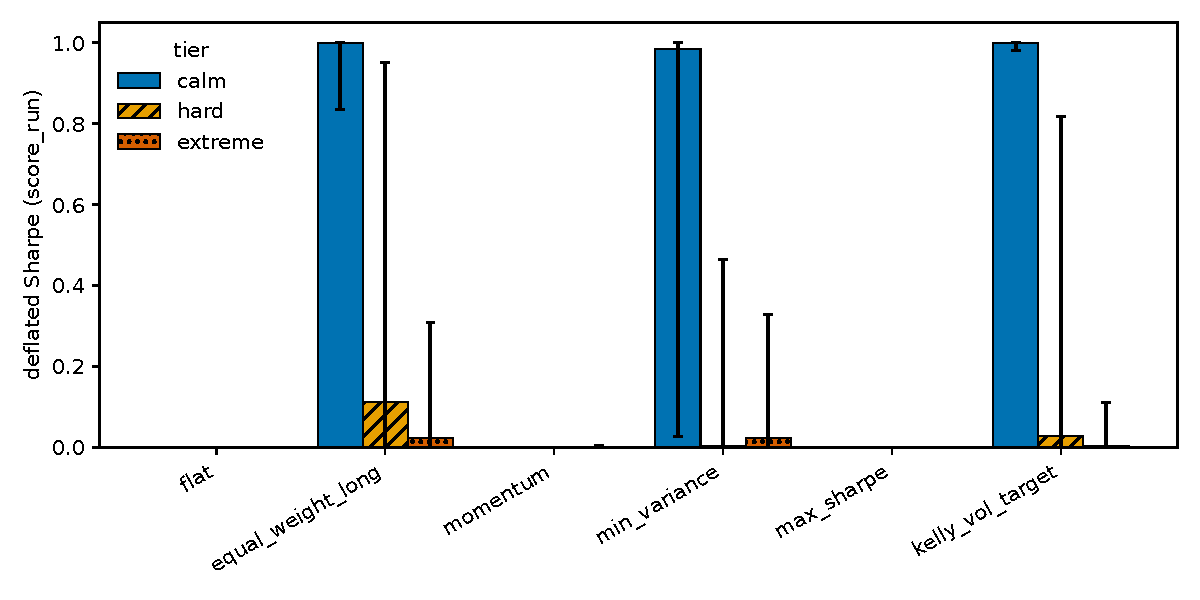
\includegraphics[width=\linewidth]{f1-baselines}
\caption{Deflated Sharpe per baseline per tier with seed-paired bootstrap CIs. Calm saturates the long baselines; Hard and Extreme collapse them toward zero.}
\label{fig:f1}
\end{figure}

\subsubsection{Rank-eligibility witness: the eligibility set is non-empty}\label{sec:witness}

The baseline board above contains no rank-eligible policy, leaving open whether the conjunction can be satisfied at all. We answer by construction with an out-of-band oracle rather than an entrant. For each seed, the script replays the deterministic, policy-invariant tape one bar ahead and mixes standardized next-bar truth $z_t$ with a seeded noise path $\varepsilon_t$:
\[
\mathrm{signal}_t(s)=s z_t+\sqrt{1-s^2}\,\varepsilon_t,
\qquad 0\le s\le1.
\]
The mixing weight $s$ is a nominal signal-strength parameter, not the realized correlation between signal and truth on a path: $z_t$ is each return divided by the episode's own sample standard deviation without centering, and $\varepsilon_t$ is one finite draw, so the per-path correlation differs from $s$. Within one noise path the same $\varepsilon_t$ is reused at every $s$ (common random numbers), so changing signal strength does not silently change the experiment. A sign-following policy trades every bar; a deadband policy trades only when $|\mathrm{signal}|>1$ and otherwise holds. Both are scored through the unchanged SharpeBench conjunction over 16 seeds. The per-run reliability gate requires every seed's PSR (\cref{sec:f1}), here against a reference Sharpe of zero, to reach $0.90$. The script records the full coarse eligibility set, the sampled strengths at which the kernel conjunction accepts. It refines an \emph{observed crossing bracket} by bisection only when that coarse set is monotone; otherwise it reports the observed set without calling any crossing a threshold. A crossing located under one noise path is a functional of that draw, so we repeat the whole procedure (coarse sweep, monotonicity check, bisection) under five independent noise paths per cell: the first is the path serialized as the primary witness, the other four redraw $\varepsilon_t$. Each bisection bracket is numerical resolution on the stated grid (half-width $0.0016$ in $s$); the spread of the crossing across noise paths is a separate, statistical quantity, and it is what \cref{tab:witness} reports. All 50 attained coarse series (10 cells, five paths each) are monotone.

\begin{table}[t]
\centering
\caption{Observed eligibility crossing in the nominal signal strength $s$: mean [min, max] of the bisection-bracket midpoint over five independent noise paths per cell. The min to max range is variation across noise realizations; the bisection bracket around each individual crossing has half-width $0.0016$ and is not shown. Crossings are found by bisection after a monotone coarse-grid check on every path, and are not global optima or theorem-level thresholds. ``none (0/5)'' means that no sampled $s\le1$ is eligible on any of the five paths. At every one of the 50 attained crossings, the last failing gate is the per-run reliability gate, the requirement that every seed's marginal PSR reach $0.90$.}
\label{tab:witness}
\small
\setlength{\tabcolsep}{3.5pt}
\begin{tabular}{llccc}
\toprule
Variant & Band & Calm & Hard & Extreme \\
\midrule
\texttt{sign\_follow} & gap-band witness & none (0/5) & $0.730\ [0.702,0.752]$ & $0.343\ [0.302,0.389]$ \\
\texttt{sign\_follow} & F1 table & none (0/5) & $0.783\ [0.764,0.820]$ & $0.353\ [0.317,0.445]$ \\
\texttt{deadband\_hold} & gap-band witness & $0.848\ [0.777,0.930]$ & $0.500\ [0.408,0.623]$ & $0.337\ [0.283,0.383]$ \\
\texttt{deadband\_hold} & F1 table & $0.690\ [0.620,0.758]$ & $0.621\ [0.483,0.755]$ & $0.342\ [0.283,0.398]$ \\
\bottomrule
\end{tabular}
\end{table}

The result is an existence proof and a calibration. The deadband construction is eligible on every tier on every noise path, so the observed eligibility set is non-empty. The per-run reliability gate is last to open at all 50 observed crossings; pooled DSR and bootstrap gates open earlier. The crossing itself is not a constant of the tier: across noise paths it moves by $0.05$ to $0.27$ in $s$ (a factor of 15 to 85 above the bisection resolution), widest for the deadband policy on Hard, so any single-path threshold is one draw from that range and the table should be read at the precision of the range rather than of the bracket. Differences between the two bands are differences between two 16-seed scenario bands as well as between noise draws, and with five paths per cell we do not test them. The sign follower never becomes eligible on Calm, on any of the five paths, because its every-bar turnover costs more than the low-volatility signal is worth; at $s=1$ the noise term vanishes, so that endpoint is noise-invariant by construction, and the failure at every $s<1$ is what the replication adds. The environment therefore imposes no activity requirement, but its cost model does require a Calm policy to ration turnover (\cref{fig:witness}).

\begin{figure}[t]
\centering
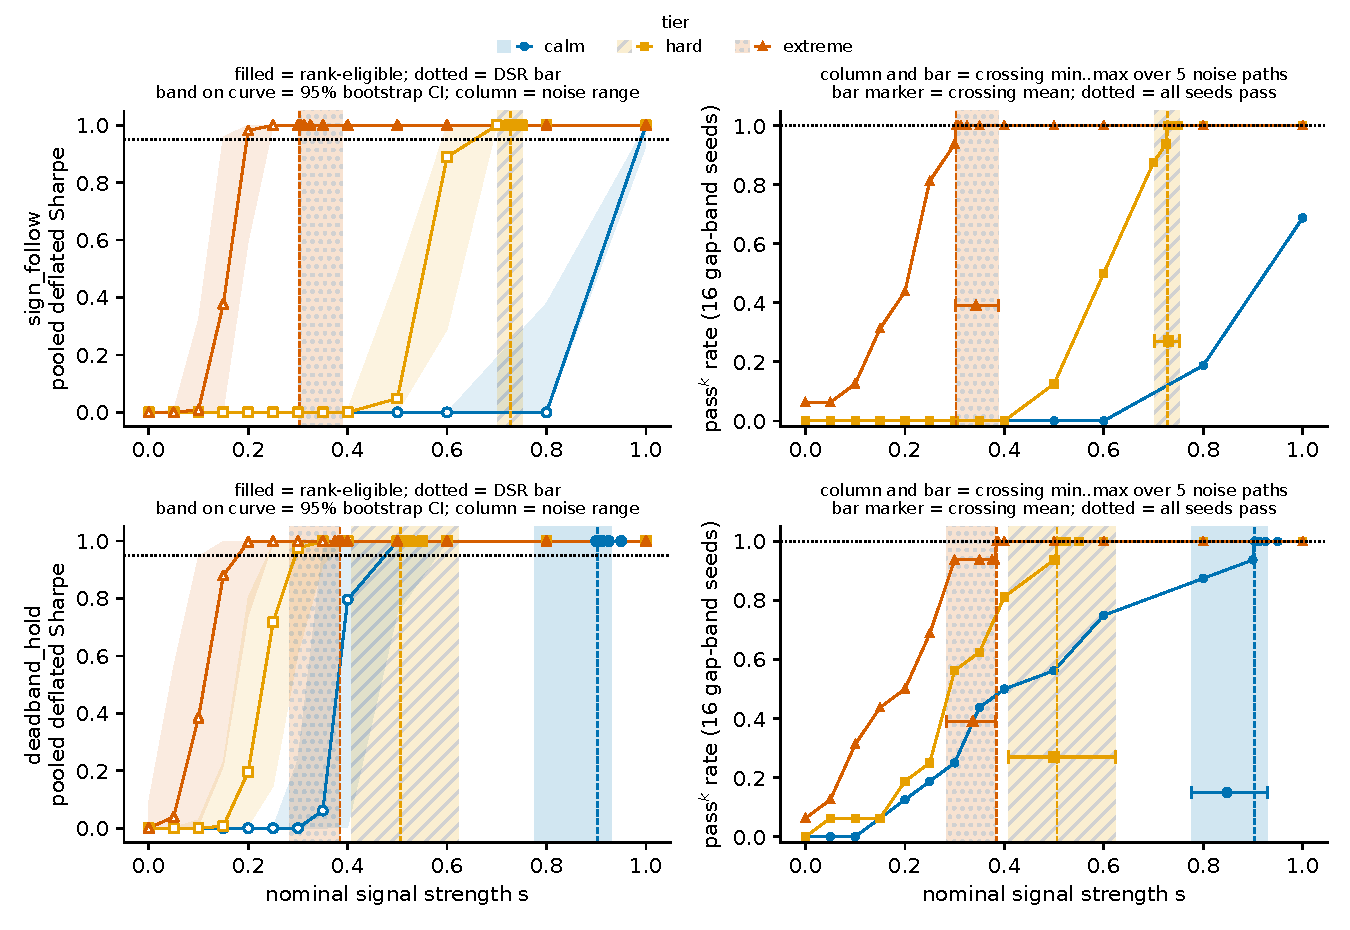
\includegraphics[width=0.95\linewidth]{witness}
\caption{Witness sweep on the gap-band witness subset under the primary noise path. Filled markers are eligible sampled points; dashed lines mark the primary-path bisection crossing, drawn only after monotonicity is verified. Shaded bands (both panels) and the horizontal bars (right panels) give the min to max range and the mean of the crossing over five independent noise paths. The right panels show how many of the 16 seed-level PSR tests pass.}
\label{fig:witness}
\end{figure}

\subsection{F2: Regret against the closed-form reference policy}\label{sec:f2}

On the Avellaneda--Stoikov market-making task, \texttt{mm\_regret} runs each candidate quoting policy and the closed-form reference policy (\cref{sec:tasks}) on the same sixteen seeded episodes ($\sigma = 2.0$, $\gamma = 0.1$, $\kappa = 1.5$, 200 steps) and reports the mean reward gap to the reference. Candidates are the reference itself and fixed-spread quoters over a grid of half-spreads. The evidence commits the per-episode regret vector per grid point; intervals are t-based 95\% CIs over the sixteen paired episodes.

The reference's regret is 0.0 by construction, which confirms the plumbing. The fixed-spread curve is U-shaped (\cref{fig:f2}): regret is 84.6 (95\% CI $[68.2, 101.1]$) at a half-spread of 0.05 (quoting too tight, filled constantly, run over by inventory), falls to a minimum of 0.037 at 0.5, and rises again to 36.6 ($[33.0, 40.2]$) at 2.0 and 58.8 ($[55.3, 62.3]$) at 4.0 (quoting too wide, earning nothing). The minimum is the point the intervals do not resolve: the 0.5 point's CI is $[-8.7, 8.8]$ and the 1.0 point's is $[-5.4, 12.4]$. Both intervals include zero, so sixteen episodes do not resolve either point from the analytical reference; this failure to reject zero is not evidence of equivalence. At the observed per-episode dispersion, sixteen paired episodes detect a mean regret of about 12 reward units at 80\% power and a two-sided 5\% level, roughly a third of the 36.6 measured at a half-spread of 2.0, so differences smaller than that are outside this design's reach. The tight and wide extremes are separated from zero by wide margins. The instrument resolves the shape of the curve, not the sign of its minimum.

The point of shipping the reference is that agents on this task are scored on regret rather than raw PnL. A market-making leaderboard ranked on PnL rewards whichever policy drew the friendliest flow; regret against a fixed analytical reference on the same episodes removes that luck axis.

\begin{figure}[t]
\centering
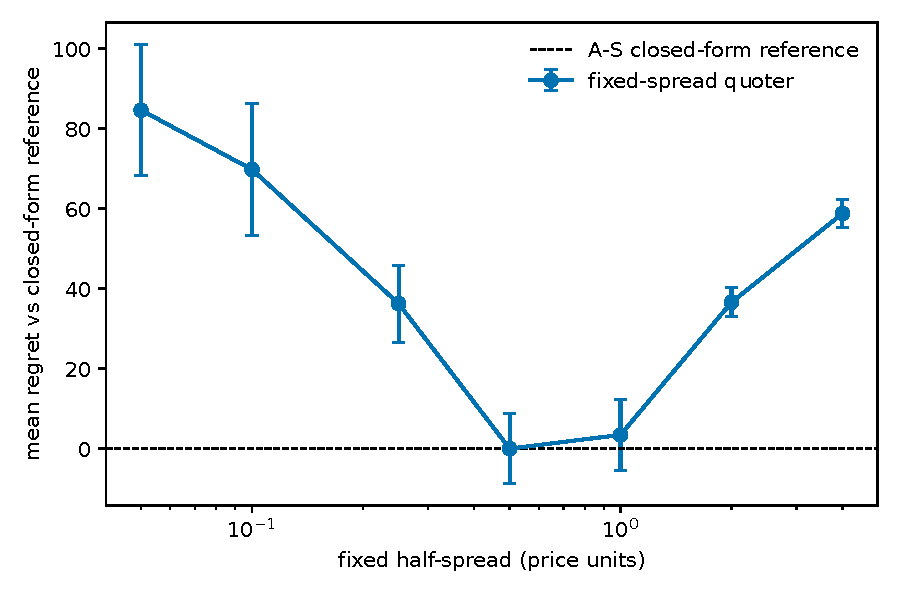
\includegraphics[width=\linewidth]{f2-regret}
\caption{Mean regret versus the analytical Avellaneda--Stoikov reference policy over 16 paired episodes, with t-based 95\% CIs. Fixed-spread quoting is U-shaped in the half-spread; the reference defines zero.}
\label{fig:f2}
\end{figure}

\subsection{F3: Generalization gap and cross-regime transfer}\label{sec:f3}

\texttt{generalization\_gap} scores the default reference policy (equal-weight long) on disjoint train and held-out seed bands (16 seeds each, separated by a 10{,}000-seed gap) within each tier. \texttt{cross\_regime\_transfer} then holds sixteen seeds fixed and varies the regime, producing the full three-by-three matrix of transfer gaps, each the in-distribution DSR minus the zero-shot out-of-distribution DSR, whose diagonal is zero by construction because identical regimes reuse byte-identical environments. The policy is fixed and parameter-free, so nothing is trained: ``source regime'' below means the regime the policy is nominally selected on, and for such a policy the matrix reduces to pairwise differences of three per-tier deflated Sharpes. Those three are the equal-weight long book's scores on the same sixteen seeds as \cref{tab:f1}, whose mean returns the two artifacts record identically, so the drift confound of \cref{sec:f1} carries over whole: on Calm drift alone saturates the score, and every transfer gap is a difference between drift-driven DSRs. What F3 measures is the instrument, how much a regime switch moves the score of a signal-free long book, and not transfer learning or the transfer of skill. These are the 16-seed subsets \cref{sec:protocol-bands} exempts fixed policies from replacing with the full canonical band. The evidence commits per-seed return series per cell; CIs are seed-resampled percentile bootstrap ($B = 2000$), seed-paired across regimes for the matrix cells.

\begin{table}[t]
\centering
\caption{Left: within-tier generalization gap (train minus test deflated Sharpe) for the fixed equal-weight reference. Right: the cross-regime transfer gap, in-distribution DSR minus zero-shot out-of-distribution DSR, with rows the source regime and columns the scored regime; a cell is a difference of two scores, not an out-of-distribution score, and the diagonal is zero by construction. Cells are read only through their seed-paired bootstrap intervals: a cell whose interval excludes zero is resolved in sign, and the Hard$\leftrightarrow$Extreme cells ($\pm 0.096$), whose intervals straddle zero, are not interpreted.}
\label{tab:f3}
\small
\begin{tabular}{lrrr}
\toprule
Tier & Train DSR & Test DSR & Gap \\
\midrule
Calm & 1.0000 & 0.9988 & $+0.0012$ \\
Hard & 0.1231 & 0.4618 & $-0.3388$ \\
Extreme & 0.0269 & 0.1280 & $-0.1012$ \\
\bottomrule
\end{tabular}
\hspace{1.5em}
\begin{tabular}{lrrr}
\toprule
 & Calm & Hard & Extreme \\
\midrule
Calm & 0.000 & $+0.877$ & $+0.973$ \\
Hard & $-0.877$ & 0.000 & $+0.096$ \\
Extreme & $-0.973$ & $-0.096$ & 0.000 \\
\bottomrule
\end{tabular}
\end{table}

\Cref{tab:f3} reports both. The within-tier gaps are the expected control: the reference policy has no fitted parameters, so it cannot overfit its train band, and the instrument correctly reads near zero on Calm ($+0.0012$) and noise-signed values on the stressed tiers (the negative Hard and Extreme gaps mean the held-out band happened to be kinder; with no learning, the gap is pure seed noise, and how much band luck a 16-seed evaluation carries is read from the interval widths rather than from any single realized gap). The per-band bootstrap intervals say the same thing at interval width: Hard's train-band DSR of 0.1231 carries a CI of $[0.000, 0.944]$ and its test band $[0.037, 0.948]$ (the bands are disjoint seed sets, so these are unpaired), overlapping almost entirely, which is what a pure-noise gap looks like. Hard's train-band DSR of 0.1231 here and \cref{tab:f1}'s 0.1114 for the same policy on the same sixteen seeds differ only in the declared trial count the deflation prior consumes, six declared policies in F1 against no declared search in the gap metric; rescoring the committed F3 return series at six trials reproduces 0.1114 exactly.

The transfer-gap matrix is where regime structure appears, and every cell is classified by one rule, fixed here for all cells: a cell whose seed-paired bootstrap interval excludes zero is resolved in sign, and the width of that interval, not the rule, says how precisely the magnitude is known. The Calm-involved point estimates are the largest: source regime Calm scored zero-shot on Hard loses $0.877$ of deflated Sharpe, and Calm to Extreme loses $0.973$ of a score bounded in $[0,1]$. Both intervals exclude zero, so both gaps are resolved in sign, but they differ in precision: Calm to Extreme is $[0.635, 0.999]$, while Calm to Hard is $[0.054, 0.999]$, which leaves its magnitude anywhere from near zero to the whole score. The Hard-to-Extreme cell ($0.096$, CI $[-0.218, 0.911]$) has an interval straddling zero, so it is not interpreted: at 16 seeds the instrument cannot distinguish it from band luck. A bounded, heavily deflated score bootstrapped over 16 seeds is a coarse instrument, which is itself a calibration result, and \cref{sec:protocol-seeds} turns it into a prescription. The matrix is antisymmetric because the policy is fixed, and its diagonal is zero by construction. Its off-diagonal magnitude is the quantity a within-tier gap is structurally blind to: a policy scored only on calm seeds can carry a saturated DSR into a leaderboard while being worth 0.03 under stress. Both metrics are cheap, and the protocol requires reporting both.

\subsection{F7: Failure-mode distributions}\label{sec:f7}

\texttt{classify\_episode\_failure} classifies every rollout of the eight-policy field (the six reference policies plus the two behavioral counterparties), across all three tiers and sixteen seeds (384 episodes), into the worst-case-first taxonomy: cascade-wiped, bankrupt, stopped-out, mandate breach (structural, drawdown or inventory), or clean, with a per-scenario sampled mandate and a 50\% drawdown stop in force. The two evidence dispositions of \cref{sec:mandates}, invalid evidence and execution failure, are counted in the same rollup and are zero on every tier, so they are omitted from \cref{tab:f7}. This artifact was regenerated for SharpeArena 0.29.0 by rerunning its producer; the other F1--F8 artifacts were not.

\begin{table}[t]
\centering
\caption{Failure-mode counts per tier, 128 episodes each (8 policies $\times$ 16 seeds). No episode reaches bankruptcy or a cascade wipe; failure is dominated by structural mandate breaches, which are flat across tiers, while the stress-sensitive modes are the drawdown family.}
\label{tab:f7}
\small
\setlength{\tabcolsep}{5pt}
\begin{tabular}{lrrrrrrr}
\toprule
Tier & Clean & Stopped out & Mandate struct. & Mandate DD & Mandate inv. & Bankrupt & Clean rate \\
\midrule
Calm & 51 & 0 & 50 & 19 & 8 & 0 & 0.40 \\
Hard & 49 & 0 & 50 & 21 & 8 & 0 & 0.38 \\
Extreme & 43 & 10 & 43 & 25 & 7 & 0 & 0.34 \\
\bottomrule
\end{tabular}
\end{table}

Mandates are sampled per scenario and assigned to fixed policies that cannot observe or adapt to them, so a structural breach is guaranteed whenever the draw pairs, say, a shorting policy with a long-only mandate. The flat structural-breach counts across tiers (50, 50, 43) are the signature of that assignment mechanism, not a behavioral finding about agents; a mandate-aware field could invert the distribution entirely, and measuring one is the interesting follow-up. The draw itself changed in SharpeArena 0.29.0: the momentum style is no longer sampled, because \texttt{mandate\_breach} reads per-bar portfolio weights and pooled returns and has no per-symbol returns to grade ``lean into recent winners'' against (\cref{sec:mandates}). Episodes that drew it in the earlier artifact are redrawn as styles that do carry a rule, so 264 of the 384 episodes are now graded against a structural constraint where 168 were before, and the structural counts rise accordingly. The remaining 120 draw the declared permissive control, which is scored by its optional caps alone and says so in its prompt text.

\Cref{tab:f7} and \cref{fig:f7} show the shape of failure as stress rises. The clean rate falls from 0.40 on Calm to 0.34 on Extreme. Each rate is 128 episodes, and the independent-binomial 95\% half-width of a difference between two such rates is about $0.12$. That width is not a floor or a ceiling for this design: episodes that share a seed or a policy are not independent, dependence does not fix the sign of their covariance, and a paired cross-tier difference over the same policies and seed indices has a covariance of its own. We therefore read the counts descriptively. Every tier-to-tier step, Calm to Extreme included at 0.40 versus 0.34, is smaller than the nominal width, and the monotone ordering of clean rates describes these 16 seeds rather than a resolved difference. What the tiers do separate is the composition of failure rather than its rate. Structural mandate breaches are flat, as the mechanism above dictates: a shorting policy under a sampled long-only mandate breaks the rule on every tier. The stress-sensitive modes are the drawdown family: mandate drawdown breaches rise from 19 on Calm to 25 on Extreme, and hard stop-outs at the 50\% line appear only on Extreme (10 episodes: 5 \texttt{overconfident}, 4 \texttt{max\_sharpe}, 1 \texttt{disposition\_effect}). No policy in this field ever reaches bankruptcy or a cascade wipe; the taxonomy's worst states are reachable but not by these baselines at this stop level. Per policy, \texttt{flat} is clean 48/48 by construction, while \texttt{overconfident} and the \texttt{momentum} policy are the worst on Calm (3 clean of 16 each, 8 of each one's failures a drawdown breach) and \texttt{overconfident} is the worst on Extreme (2 clean of 16). On this mandate-blind reference field, most episodes end in a process failure that a return-ranked board does not record: 231 of 384. Counted against failures rather than episodes the share is 231 of 241, because only ten episodes fail on PnL at all, every one of them a stop-out.

\begin{figure}[t]
\centering
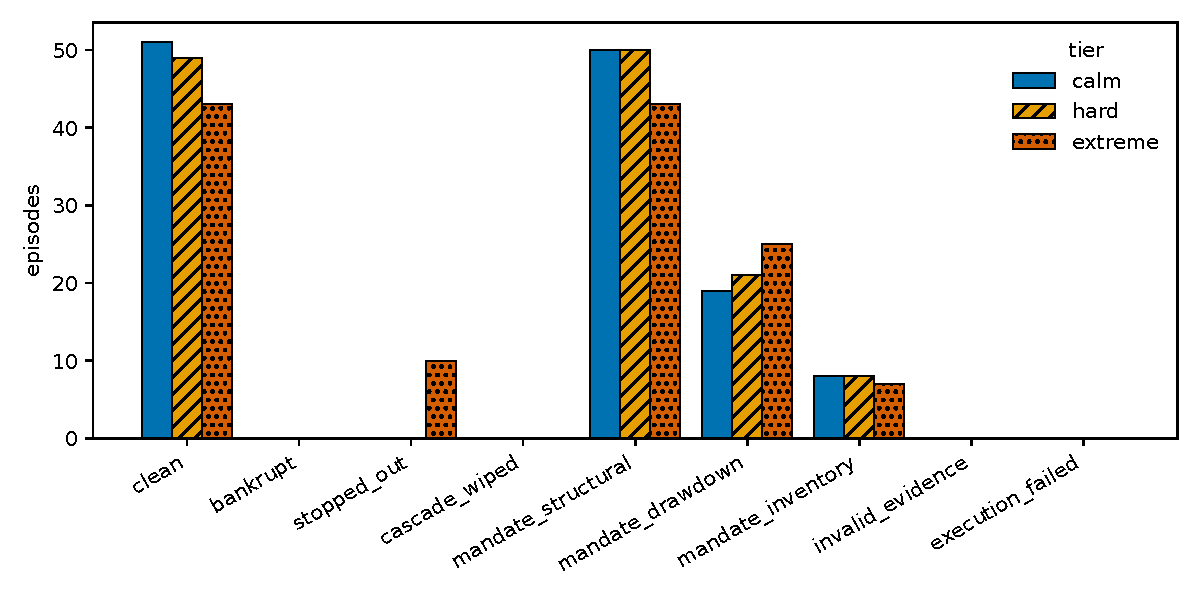
\includegraphics[width=\linewidth]{f7-failures}
\caption{Failure-mode distribution per tier per policy over 384 classified episodes.}
\label{fig:f7}
\end{figure}

\subsection{F8: Ecology outcomes under shocks, replicated over seeds}\label{sec:f8}

\texttt{run\_ecology} seeds the replicator with the eight baseline species over a shared-book market via \texttt{market\_payoffs} (12 generations, field size 8, innovation every 4 generations breeding parameter-perturbed variants of the leader) and runs trajectories under a steady all-Calm control schedule and a \texttt{regime\_shocks} schedule rotating Calm (generations 0 to 3), Hard (4 to 7) and Extreme (8 to 11). We replicate the probe over eight replicator seeds per schedule; \cref{tab:f8} reports the cross-seed winner distribution, and the seed-0 trajectories (\cref{fig:f8}) remain the illustrative detail. The two schedules chain episode seeds differently (the shock schedule strides seeds across generations), so control and shocked runs at the same replicator seed are matched in configuration, not in price paths.

The replicator flow rule sits in the market-ecology tradition: strategies as species whose profitability decays as their share of the flow grows \citep{farmer2002market}, and populations whose composition, rather than any single agent's optimization, drives aggregate dynamics \citep{lux1999scaling}. The implementation abstracts away much of what those models study: capital flows react instantly (no fund-flow lags), there are no leverage or margin constraints beyond the strategies' own sizing, and there is no entry beyond the single leader-perturbation innovator. Its outputs are trajectories of this replicator map, not claims about market ecology in general.

\begin{table}[t]
\centering
\caption{Replicated ecology outcomes over 8 replicator seeds per schedule: distribution of the final dominant lineage (bred variants credited to their founding species). The root winner differs between the schedules on 5 of 8 seeds, and on 3 of the 6 seeds where both schedules resolve a dominant lineage; the seed-0 replacement of the volatility targeter by the equal-weight long book occurs on 1 of 8 seeds.}
\label{tab:f8}
\footnotesize
\setlength{\tabcolsep}{4pt}
\begin{tabular}{lrr}
\toprule
Final dominant lineage & Control (all Calm) & Shocked (Calm/Hard/Extreme) \\
\midrule
kelly\_vol\_target & 4 & 7 \\
equal\_weight\_long & 2 & 1 \\
flat (no resolved dominant) & 2 & 0 \\
\bottomrule
\end{tabular}
\end{table}

The replication does not support the single-seed narrative. At seed 0 the story was clean: \texttt{kelly\_vol\_target} sweeps the control board (peak share 1.00, final 0.81), collapses under the shock schedule once the regime turns Hard, and \texttt{equal\_weight\_long} inherits dominance (final 0.67). Across eight seeds that story is the exception. Under the shock schedule a \texttt{kelly\_vol\_target} lineage ends dominant on 7 of 8 seeds (final shares near 0.90); the seed-0 handoff to the long book happens once. The control side is itself seed-dependent: \texttt{kelly\_vol\_target} wins 4 seeds, \texttt{equal\_weight\_long} wins 2, and on 2 seeds no species resolves dominance at all (all eleven end persistent at small shares, with a \texttt{flat} variant holding the largest share at 0.10). The root-level winner differs between the two schedules on 5 of 8 seeds, but on 2 of those the control side never resolves a dominant lineage at all; among the 6 seeds where both schedules resolve one, the winner differs on 3. At eight seeds the reordering is neither established nor excluded, and it has no consistent direction. Extinction pressure is more stable than identity: shocked runs produce a resolved dominant on 8/8 seeds with 4 to 7 extinctions per run (at seed 0, both behavioral counterparties are gone or collapsed on both schedules, \texttt{overconfident} extinct at generation 0).

One replicator trajectory is one draw from a heavy-tailed outcome distribution, and single-run ecology narratives do not survive replication. What the probe reliably produces at this scale is the outcome distribution itself: which lineages can win, how often shocks reorder the board, and how much of the population goes extinct, per committed seed set. Sharper claims need more seeds, varied shock orderings and path-matched schedule pairs, all of which are mechanical extensions of the committed script.

\begin{figure}[tbp]
\centering
\begin{subfigure}[t]{0.92\linewidth}
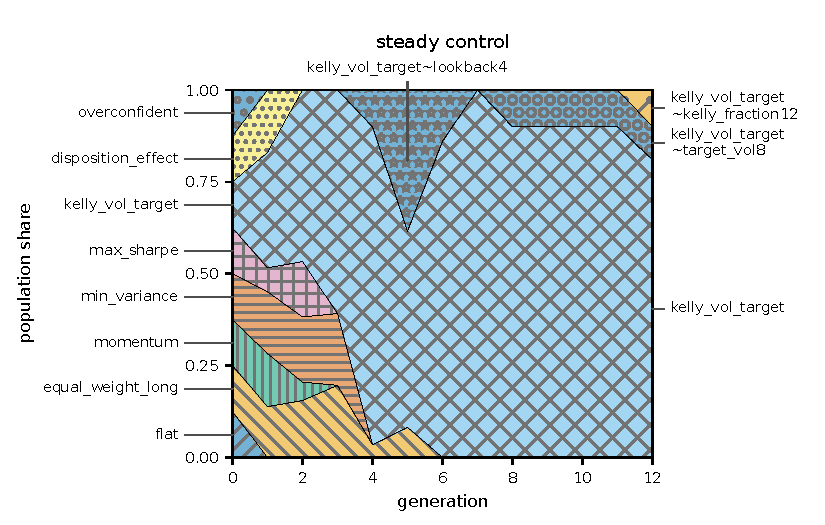
\includegraphics[width=\linewidth]{f8-ecology-control}
\caption{Control: steady Calm.}
\end{subfigure}

\vspace{0.8em}

\begin{subfigure}[t]{0.92\linewidth}
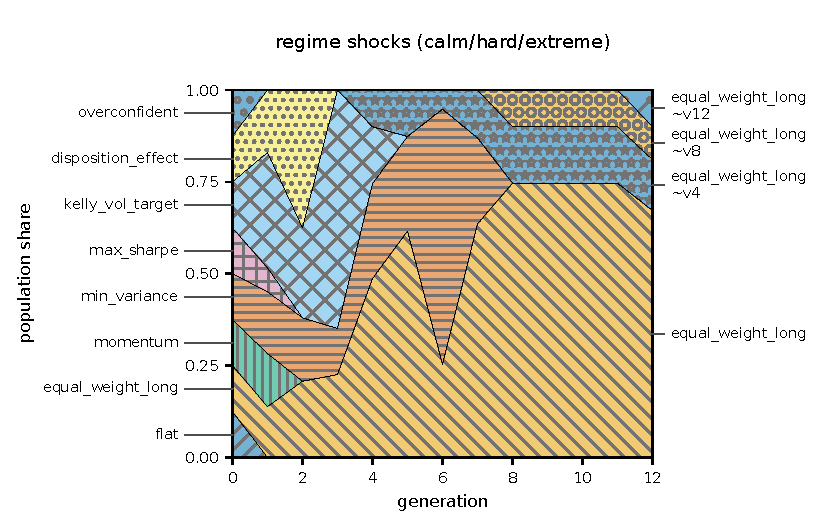
\includegraphics[width=\linewidth]{f8-ecology-shocked}
\caption{Shocked: Calm, then Hard, then Extreme.}
\end{subfigure}
\caption{Seed-0 population-share trajectories over 12 replicator generations, the illustrative single run behind \cref{tab:f8}'s distribution. Each band is one species' share, labelled directly on the plot and separated from its neighbours by hatching, so no band is identified by a legend alone. At this seed the regime rotation replaces the calm-regime winner with the equal-weight long book; across the eight-seed replication that replacement occurs once.}
\label{fig:f8}
\end{figure}

\input{sections/09-related}
\input{sections/10-limitations}
\section{Conclusion}\label{sec:conclusion}

\paragraph{What the environment establishes.} The environment's guarantees are properties of committed code, each checkable by a listed test (\cref{app:commands}). The data layer has no operation that returns a bar past the cursor. The determinism-critical core reproduces committed goldens on the native, WebAssembly and packaged surfaces. Replay recomputes performance from recorded decisions and frozen engine inputs, so a doctored decision stream does not reproduce the honest run. The checked and repository scoring paths turn a recorded wire fault into a typed failed cell rather than a hold. Each guarantee has a stated boundary (\cref{sec:limitations}): leak-freedom at the interface is not an information guarantee, the Python probe layer sits outside the golden-hash path, and replay does not authenticate every trace field.

\paragraph{What the probes establish.} The probes establish less, and several of their results go against the environment. The canonical generator fails its own finite-panel-calibrated realism conjunction on 23 of 24 seeded panels, and a predeclared Calm sweep finds no setting that survives its rule (\cref{sec:f4,sec:calm-tails}). No reference policy is rank-eligible, while an out-of-band oracle shows that the eligibility set is non-empty on every tier (\cref{sec:f1,sec:witness}). On the market-clearing models the symmetric pump loses money at every sampled coefficient, an asymmetric schedule under concave impact pays on sampled cells without follower flow, and makers keep a positive markout against informed flow at the default calibration (\cref{sec:f5,sec:f6}). A public bounded seed band is inverted from one observed bar, and the sealed derivation defeats that scanner (\cref{sec:predictability,sec:sealed-seeds}). The single-seed ecology narrative does not survive replication (\cref{sec:f8}). Every one of these numbers calibrates an instrument with fixed reference policies, on tape or on specified models the paper does not claim are market-valid.

\paragraph{What stays open.} Two questions remain open, and neither is answered by rereading the committed evidence. The first is learning. No agent is trained here, the near-zero within-tier generalization gaps are the expected control for policies with nothing to overfit, and no current-model field has been admitted, so what a trained or model agent scores, and whether the seed-band protocol separates its skill from band luck, is future evidence. The second is market validity. The canonical tape sits at the lowest level of the empirical-validity scheme on the axis the realism gate grades, the impact models are stylized, and the market-making and market-clearing simulators are calibrations of specified models rather than validated markets. SharpeArena offers a producer whose present guarantees can be checked without trusting its authors, and diagnostics that report where its tape is not yet market-like; closing either open question requires a new experiment rather than a new reading of the old ones.

\input{sections/12-reproducibility}
\section{Ethics and broader impact}\label{sec:ethics}

\paragraph{Dual-use surfaces.} Three parts of this release can be turned against the purpose they were built for. The manipulation probe of \cref{sec:f5} is a payoff-search harness over trade-based manipulation schedules \citep{allen1992stock}, and is dual-use by construction. The in-band inversion probe of \cref{sec:predictability} publishes a scan that recovers a scenario's seed, and with it every future bar, from one observed bar of a public bounded seed band in about one second. And a byte-verifiable leaderboard score is more persuasive than an unverifiable one without being more externally valid.

\paragraph{The profitable manipulation cells.} The paper reports manipulation schedules that pay, and states where. Every sampled coefficient of the symmetric linear sweep loses money, and so does every one of the 45 sampled linear cells of the asymmetric search, which is consistent with the no-manipulation conditions of the linear model under its assumptions. Under normalized concave permanent impact at $\beta=0.5$, slow accumulation followed by block liquidation pays on the two arms without follower flow: four of the 135 cells keep familywise-positive intervals, the selected cell replicates on 32 fresh seeds, and the extended sweep's largest sampled cell is a longer trip of the same shape; the canonical follower arm has no pointwise-positive cell (\cref{sec:f5-positive-control,sec:f5-extended-sweeps}). These are statements about a stylized simulator at one calibration, gross of fees, in discrete time with no latency and with a one-parameter follower population. They are not estimates of what any schedule earns in a market.

\paragraph{What is and is not released.} Released: the environment, the probe modules, the producer scripts and the committed per-cell evidence behind every reported number, the manipulation grid included, in the public repository under the MIT and Apache-2.0 licenses, with the environment and probe modules also in the published packages. Not released, because none exists: a real-market price series inside the environment, a trained policy, model weights, an admitted model-performance result, an execution path from the manipulation module to any order adapter, and a real-capital endpoint. Inside the Python package the manipulation module is imported only by the package namespace, not by the forward paper arm, and that arm's order adapter refuses every origin other than a paper-trading endpoint (\cref{sec:forward-paper}). The module's own documentation states that it is a simulator diagnostic and not a strategy, that its schedules are written to be crude and obvious, and that no output of it should be handed to an execution surface. That is a stated norm, not an enforced one.

\paragraph{Misuse.} We name three misuses. The first is presenting a SharpeArena score, verified or not, to investors or retail audiences as evidence of real-market skill: a verified number is a claim about a synthetic environment only, and SharpeArena scores are not performance marketing. The second is reading the profitable concave cells as a trading recipe, or fitting or deploying schedules taken from the manipulation module. The third is running the seed-band scan against an evaluation one has entered, which the protocol forbids (\cref{sec:protocol-custody}). No license term enforces any of the three; this section states them as norms.

\paragraph{Why we publish the probes.} We judge publishing them net positive. The linear arm is a diagnostic against a stated no-manipulation assumption rather than a search for deployable trades, and the paper makes no guarantee outside its finite grid. The concave positive control shows that the instrument can see a paying schedule, which a probe that has never returned a positive cannot claim. Publishing the seed scan beside the sealed-seed derivation of \cref{sec:sealed-seeds} turns an attack a motivated entrant could run silently into a documented threat with a shipped mitigation.

\paragraph{Data and people.} No human subjects and no personal data are involved. The environment's tape is synthetic, and the forward paper arm reads public market data read-only. No model inference contributes to any admitted result; the use of language models in preparing the manuscript is stated in \cref{sec:declarations}.


\bibliographystyle{plainnat}
\bibliography{refs}

\appendix
\section{Commands that produce every number}\label{app:commands}

All commands run from the repository root at the tagged version, with the \texttt{sharpearena} Python package installed. The package version is recorded in every evidence file (\texttt{sharpearena} 0.8.0 over the SharpeBench 0.5.0 kernel for this run). Each evidence script fixes its seeds internally, writes JSON to \texttt{paper/evidence/} and, where a figure carries the finding, a PDF to \texttt{paper/figures/}.

\paragraph{The design-property checks (\cref{sec:leakfree,sec:determinism,sec:replay,sec:contract}).}
\begin{verbatim}
cargo test -p sharpearena              # golden hashes, leak-free
                                       # property tests, conformance kit
cargo test -p sharpearena-wasm         # native == wasm parity + golden
npm test --prefix npm/sharpearena      # replay + tamper detection
python -m pytest crates/sharpearena-py # Python surface, check_env,
                                       # seed-band disjointness
\end{verbatim}

\paragraph{F1: baseline leaderboard (\cref{sec:f1}).}
\begin{verbatim}
python paper/src/make-f1-baselines.py
  -> paper/evidence/f1-baselines.json, paper/figures/f1-baselines.pdf
\end{verbatim}

\paragraph{F2: regret vs the closed-form optimum (\cref{sec:f2}).}
\begin{verbatim}
python paper/src/make-f2-regret.py
  -> paper/evidence/f2-regret.json, paper/figures/f2-regret.pdf
\end{verbatim}

\paragraph{F3: generalization gap and cross-regime transfer (\cref{sec:f3}).}
\begin{verbatim}
python paper/src/make-f3-generalization.py
  -> paper/evidence/f3-generalization.json,
     paper/figures/f3-transfer-matrix.pdf
\end{verbatim}

\paragraph{F4: stylized-facts realism certification (\cref{sec:f4}).}
\begin{verbatim}
python paper/src/make-f4-realism.py
  -> paper/evidence/f4-realism.json, paper/figures/f4-realism.pdf
\end{verbatim}

\paragraph{F5: manipulation boundary and size response (\cref{sec:f5}).}
\begin{verbatim}
python paper/src/make-f5-manipulation.py
  -> paper/evidence/f5-manipulation.json,
     paper/figures/f5-boundaries.pdf, paper/figures/f5-size-response.pdf
\end{verbatim}

\paragraph{F6: adverse-selection markouts (\cref{sec:f6}).}
\begin{verbatim}
python paper/src/make-f6-adverse-selection.py
  -> paper/evidence/f6-adverse-selection.json,
     paper/figures/f6-markouts.pdf
\end{verbatim}

\paragraph{F7: failure-mode distributions (\cref{sec:f7}).}
\begin{verbatim}
python paper/src/make-f7-failures.py
  -> paper/evidence/f7-failures.json, paper/figures/f7-failures.pdf
\end{verbatim}

\paragraph{F8: ecology under shocks (\cref{sec:f8}).}
\begin{verbatim}
python paper/src/make-f8-ecology.py
  -> paper/evidence/f8-ecology.json,
     paper/figures/f8-ecology-control.pdf,
     paper/figures/f8-ecology-shocked.pdf
\end{verbatim}

\paragraph{Regenerating every figure from the committed evidence.}
\begin{verbatim}
python paper/src/make-figures.py
\end{verbatim}
Each \texttt{make-f*} script produces its own figure at run time; \texttt{make-figures.py} re-renders all figures from the JSON already in \texttt{paper/evidence/} without re-running any experiment, so a reader can check that no figure contains a number the evidence does not.


\end{document}
